
\chapter{Étude phénoménologique} \label{chap:chap2}

\begin{fmffile}{chapitre2}

\section{Le quark top}\label{sec:quarktop}

Le quark top est la particule élémentaire la plus massive connue à ce jour. Sa masse très élevée en fait un candidat très sérieux à la découverte de physique nouvelle. En effet, si les couplages de nouvelle physique suivent les même tendances que le couplage de Yukawa, c'est-à-dire d'autant plus intense que la masse de la particule en jeu est élevée, il est alors attendu de voir se manifester des phénomènes autour du quark top préférentiellement.
\begin{equation}
m_t^\textrm{Tevatron + LHC} =  \SI{172.76 \pm 0.30}{\GeV} \cite{PDG}
\end{equation}

Le quark top a été découvert en 1995 au Tevatron par les expériences CDF et $D\emptyset$. Cependant, son existence fut prédite plusieurs années avant son observation.
Le quark b, découvert en 1977, se désintègre par interaction faible. Il appartient donc à un doublet $SU(2)_L$, dont le partenaire est le quark top.

Le LHC est une usine à top, il est donc un collisionneur idéal pour l'étude des théories au-delà du Modèle Standard. Dans cette section, est présenté un résumé des propriétés du quark top.

\subsection{Production du quark top au LHC} 
\subsubsection{Production par paire}
Dans les collisionneurs hadroniques tels que le LHC, la production dominante est la production par paire de quark top-antitop (production \ttbar). Au LHC Run II à $\sqrt{s} =$ \SI{13}{\TeV} la section efficace est $\sigma_{\ttbar} =$ \SI{831.8}{\pico\barn}, calculée au next-to-next-leading order (NNLO) de la QCD perturbative, avec une incertitude relative d'environ \SI{6}{\%} \cite{mitov}. 
Le PDF du gluon est très important à $Q \sim m_{\Ptop}$, c'est-à-dire que ce sont des gluons qui seront majoritairement représentés dans les collisions. 
Du fait de la différence entre les PDF des quarks et des gluons dans le proton aux  énergies du LHC, les modes sont distribués avec  \SI{88.6}{\%} de production par fusion de gluons contre \SI{11.4}{\%} par annihilation quark-antiquark. La figure \figurename{\ref{fig:ttbar_diagrams}} résume les diagrammes de Feynmann des différents modes de production de paires \ttbar.


\begin{figure} \centering
    \subcaptionbox{\label{fig:ttbar_fusion_gluon_1}}[0.3\textwidth]{
    \begin{fmfgraph*}(160,70)
        \fmfpen{0.5}
        \fmfleft{i1,i2}
        \fmfright{o1,o2}
        \fmf{gluon}{i1,v1,i2}
        \fmf{gluon}{v1,v2}
        \fmf{fermion}{o1,v2,o2}
        \fmfdot{v1,v2}
        \fmflabel{$t$}{o2}
        \fmflabel{$\bar{t}$}{o1}
    \end{fmfgraph*}
    }\hfill
    \subcaptionbox{\label{fig:ttbar_fusion_gluon_2}}[0.3\textwidth]{
    \begin{fmfgraph*}(160,70)
        \fmfpen{0.5}
        \fmfleft{i1,i2}
        \fmfright{o1,o2}
        \fmf{gluon}{i1,v1}
        \fmf{gluon}{i2,v2}
        \fmf{fermion}{o1,v1}
        \fmf{fermion}{v2,o2}
        \fmf{fermion,tension=1}{v1,v2}
        \fmfdot{v1,v2}
        \fmflabel{$t$}{o2}
        \fmflabel{$\bar{t}$}{o1}
    \end{fmfgraph*}
    } \hfill
    \subcaptionbox{\label{fig:ttbar_qq}}[0.3\textwidth]{
    \begin{fmfgraph*}(160,70)
        \fmfpen{0.5}
        \fmfleft{i1,i2}
        \fmfright{o1,o2}
        \fmf{fermion}{i1,v1,i2}
        \fmf{gluon}{v1,v2}
        \fmf{fermion}{o1,v2,o2}
        \fmfdot{v1,v2}
        \fmflabel{\Pquark}{i1}
        \fmflabel{\APquark}{i2}
        \fmflabel{\Ptop}{o2}
        \fmflabel{\APtop}{o1}
    \end{fmfgraph*}
    }\hfill
    \caption{Diagrammes de Feynman de production de paires \ttbar par fusion de gluons (\subref{fig:ttbar_fusion_gluon_1}, \subref{fig:ttbar_fusion_gluon_2}), ainsi que par annihilation de quarks (\subref{fig:ttbar_qq}).}
    \label{fig:ttbar_diagrams}
\end{figure}

\subsubsection{Production célibataire}\label{topcelibataire}

Un deuxième mode de production permet de produire des quarks top célibataires, \emph{via} l'interaction faible. Trois canaux de production existent à l'arbre, présentés dans les figures  \figurename{\ref{fig:singletop_diagrams}}, \figurename{\ref{fig:singletop_diagrams_2}}. Le diagramme \figurename{\ref{fig:single_top_t_channel}}, connu sous le nom de voie t, est le processus dominant, avec une section efficace NNLO approché de $\sigma_{\Ptop + \APtop} =$ \SI{215}{\pico\barn} avec une incertitude relative d'environ \SI{1}{\%} \cite{singletopNNLO}. 

Les deux autres canaux sont la voie s (\figurename{\ref{fig:single_top_s_channel}}) et la production associée d'un quark top et d'un boson \PW (voie \Ptop{}\PW{} \figurename{\ref{fig:singletop_diagrams_2}}).


\begin{figure} \centering
    \subcaptionbox{\label{fig:single_top_s_channel}}[0.48\textwidth]{
    \fmfframe(0,10)(0,0){\begin{fmfgraph*}(160,70)
        \fmfpen{0.5}
        \fmfleft{i1,i2}
        \fmfright{o1,o2}
        \fmf{fermion}{i1,v1,i2}
        \fmf{boson,label=\PWplus}{v1,v2}
        \fmf{fermion}{o1,v2,o2}
        \fmfdot{v1,v2}
        \fmflabel{\Pquark}{i1}
        \fmflabel{\APquark}{i2}
        \fmflabel{\Ptop}{o2}
        \fmflabel{\APbottom}{o1}
    \end{fmfgraph*}}
    }\hfill
    \subcaptionbox{\label{fig:single_top_t_channel}}[0.48\textwidth]{
    \fmfframe(0,10)(0,0){\begin{fmfgraph*}(160,70)
        \fmfpen{0.5}
        \fmfleft{i1,i2}
        \fmfright{o1,o2}
        \fmf{fermion}{i1,v1,o1}
        \fmf{fermion}{i2,v2,o2}
        \fmf{boson,label=\PWplus}{v1,v2}
        \fmfdot{v1,v2}
        \fmflabel{\Ptop}{o1}
        \fmflabel{\Pbottom}{i1}
        \fmflabel{$\Pquark^\prime$}{o2}
        \fmflabel{\Pquark}{i2}
    \end{fmfgraph*}}
    }
    \caption{Diagrammes de Feynman de la production de quark top célibataire, en voie s (\subref{fig:single_top_s_channel}) et en voie t (\subref{fig:single_top_s_channel})}
    \label{fig:singletop_diagrams}
\end{figure}


\begin{figure} \centering
    \subcaptionbox{}[0.48\textwidth]{
    \begin{fmfgraph*}(160,70)
        \fmfpen{0.5}
        \fmfleft{i1,i2}
        \fmfright{o1,o2}
        \fmf{fermion}{i1,v1}
        \fmf{fermion,label=\Pbottom}{v1,v2}
        \fmf{gluon}{i2,v1}
        \fmf{boson}{v2,o2}
        \fmf{fermion}{v2,o1}
        \fmfdot{v1,v2}
        \fmflabel{\Ptop}{o1}
        \fmflabel{\APbottom}{i1}
        \fmflabel{\PWplus}{o2}
    \end{fmfgraph*}
    }\hfill
    \subcaptionbox{}[0.48\textwidth]{
    \begin{fmfgraph*}(160,70)
        \fmfpen{0.5}
        \fmfleft{i1,i2}
        \fmfright{o1,o2}
        \fmf{fermion}{i1,v1}
        \fmf{fermion,label=$t$}{v1,v2}
        \fmf{gluon}{i2,v2}
        \fmf{boson}{v1,o1}
        \fmf{fermion}{v2,o2}
        \fmfdot{v1,v2}
        \fmflabel{$t$}{o2}
        \fmflabel{$b$}{i1}
        \fmflabel{\PWplus}{o1}
    \end{fmfgraph*}
    }
    \caption{Diagrammes de Feynman de la production associée d'un quark top célibataire et d'un boson \PW (voie \Ptop{}\PW{}).}
    \label{fig:singletop_diagrams_2}
\end{figure}


\subsection{Désintégration du quark top.} 

La durée de vie mesurée du quark top est d'environ \SI{3.3e-25}{\s} \cite{PDG}. Ce temps de vie est inférieur au temps d'hadronisation ($\tau_{\textrm{hadronisation}} \simeq $ \SI{3e-24}{\s}) ce qui implique que le quark top se désintègre avant de s'hadroniser. Il offre donc une possibilité unique d'étudier un quark dans un état non-lié.

Le quark top se désintègre uniquement par interaction faible, selon trois modes de désintégration : $\Ptop \rightarrow \Pbottom \PWplus$, $\Ptop \rightarrow \Pstrange \PWplus$ et $\Ptop \rightarrow \Pdown \PWplus$. La mesure de la matrice CKM \eqref{CKM} montre que le terme $|V_{tb}|^2 = $ \SI{0.999172 \pm 0.000024} est hautement dominant. Ainsi, le quark top se désintègre majoritairement en $\Ptop \rightarrow \Pbottom \PWplus$.

L'état final exact de la désintégration du quark top dépend du \PW, qui se désintègre environ \SI{33}{\%} du temps en lepton - neutrino, et \SI{67}{\%} en paire de quark-antiquark. Les rapports d'embranchements de la désintégration du \PW sont résumés dans la table \tablename{\ref{desintegration}}.

\begin{table}
\begin{center}
\begin{tabular}{cc}
    \noalign{\smallskip}\hline\noalign{\smallskip}
    Canal & Rapport d'embranchement $(\Gamma_i / \Gamma)$ \\
    \noalign{\smallskip}
    \hline \hline
    \noalign{\smallskip}
    \Pelectron + \Pnue& \SI{11.10 \pm 0.30}{\%}   \\
    \Pmuon + \Pnum& \SI{11.40 \pm 0.20}{\%}\\
    \Ptau + \Pnut & \SI{11.10 \pm 0.90}{\%} \\
    \Pquark{}\APquark{} & \SI{66.5 \pm 1.4}{\%}\\
    \noalign{\smallskip}\hline\noalign{\smallskip}
\end{tabular}
\caption{Rapports d'embranchements des différents canaux de désintégration du boson \PW \cite{PDG}.}
\label{desintegration}
\end{center}
\end{table}


Lors d'une production par paire, les deux quarks top vont se désintégrer de façon indépendante. Le \PW ayant 4 modes de désintégration, l'état final d'une désintégration \ttbar peut être classé en 3 catégories :
\begin{itemize}
    \item Les deux \PW se désintègrent en \Plepton + \Pnulepton (avec \Plepton un lepton quelconque). On parle alors de désintégration di-leptonique (canal di-lepton).
    \item Un \PW se désintègre en \Plepton + \Pnulepton, et le deuxième en  \Pquark{}\APquark{}. C'est le canal semi-leptonique, aussi appelé lepton + jets.
    \item Finalement, les deux \PW peuvent aussi se désintégrer en \Pquark{}\APquark{}. On parle dans ce cas de canal tout-hadronique.
 \end{itemize}

\begin{figure}
    \centering
    \subcaptionbox{\label{fig:top_pair_decay_channels}}[0.45\textwidth]{
    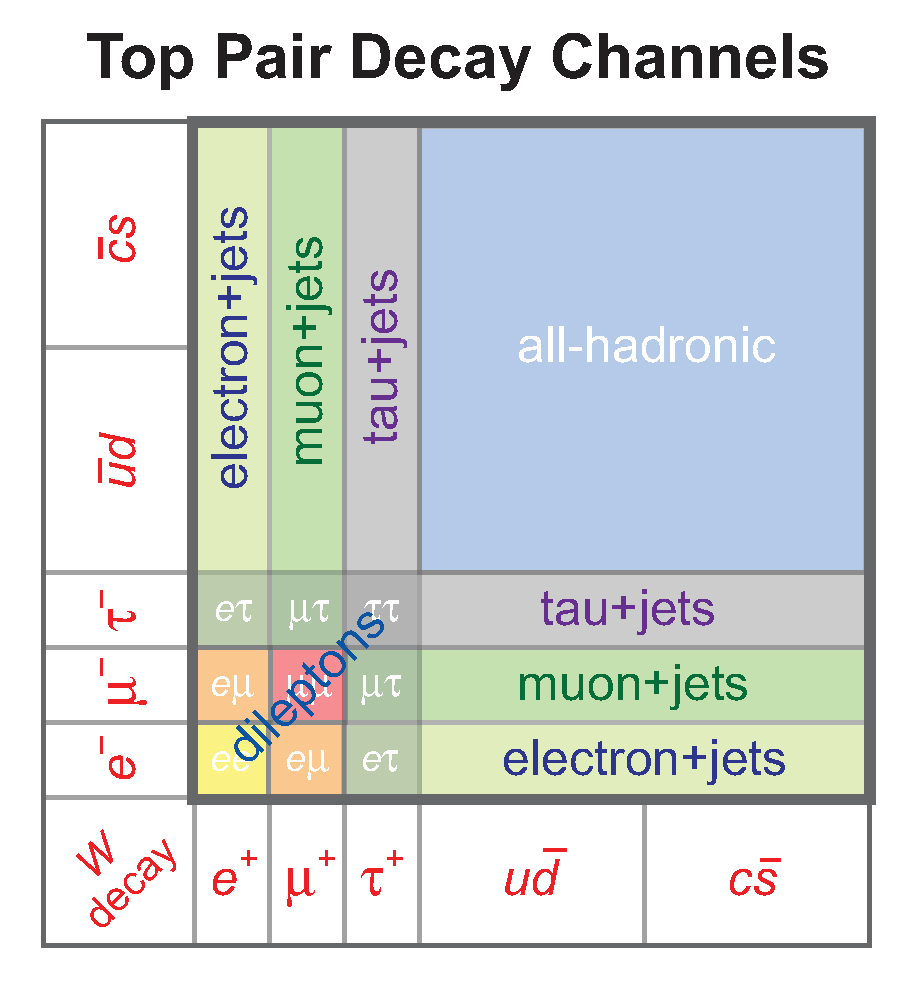
\includegraphics[width=0.40\textwidth]{top_pair_decay_channels.pdf}
    } 
    \qquad
    \subcaptionbox{\label{fig:top_pair_branching_frac}}[0.45\textwidth]{
    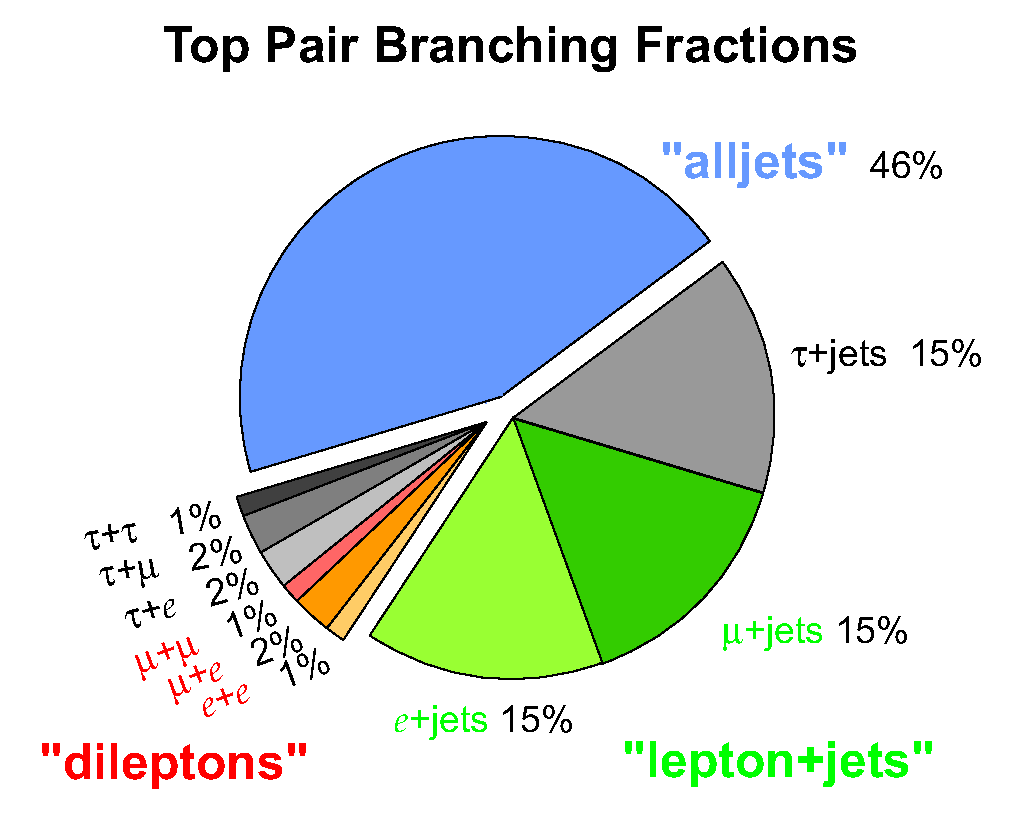
\includegraphics[width=0.45\textwidth]{top_pair_branching_frac.pdf}
    }
    \caption{Canaux de désintégration d'une paire \ttbar (\subref{fig:top_pair_decay_channels}) et rapports d'embranchements des différents canaux de désintégration d'une paire \ttbar (\subref{fig:top_pair_branching_frac}).}
\end{figure}

Cette classification est résumée dans la figure \figurename{\ref{fig:top_pair_decay_channels}}. Les rapports d'embranchements associés à chaque canal de désintégration sont résumés \figurename{\ref{fig:top_pair_branching_frac}}. On constate ainsi qu'environ \SI{46}{\%} des paires \ttbar se désintègrent dans le canal tout-hadronique, \SI{\sim 45}{\%} dans le canal semi-leptonique, et \SI{\sim 9}{\%}  dans le canal di-leptonique. Les diagrammes de Feynman associés à ces désintégrations sont présentés dans la figure \figurename{\ref{fig:top_pair_decay_feynman}}.

\begin{figure}
    \centering
    \subcaptionbox{\label{fig:top_pair_decay_dileptonic}}[0.48\textwidth]{\begin{fmfgraph*}(180,150)
        \fmfpen{0.5}
        \fmfleft{t1,i1,i2,t2}
        \fmfright{o1,o2,o3,o4,o5,o6}

        \fmf{gluon}{i1,v1,i2}
        \fmf{gluon}{v1,v2}
        \fmf{fermion,label=\APtop,label.side=left}{v3,v2}
        \fmf{fermion,label=\Ptop,label.side=left}{v2,v4}
        \fmf{boson,label=\PWplus,label.side=left}{v4,v6}
        \fmf{boson,label=\PWminus,label.side=right}{v3,v5}
        \fmf{fermion}{v5,o1}
        \fmf{fermion}{o6,v6}

        \fmffreeze

        \fmf{fermion}{o3,v3}
        \fmf{fermion}{v4,o4}

        \fmf{fermion}{v6,o5}
        \fmf{fermion}{o2,v5}

        \fmflabel{\Pleptonminus}{o1}
        \fmflabel{\APnulepton}{o2}

        \fmflabel{\APbottom}{o3}
        \fmflabel{\Pbottom}{o4}

        \fmflabel{\Pnulepton}{o5}
        \fmflabel{\Pleptonplus}{o6}

        \fmfdot{v1,v2,v3,v4,v5,v6}
    \end{fmfgraph*}}\hfill
    \subcaptionbox{\label{fig:top_pair_decay_semileptonic}}[0.48\textwidth]{\begin{fmfgraph*}(180,150)
        \fmfpen{0.5}
        \fmfleft{t1,i1,i2,t2}
        \fmfright{o1,o2,o3,o4,o5,o6}

        \fmf{gluon}{i1,v1,i2}
        \fmf{gluon}{v1,v2}
        \fmf{fermion,label=\APtop,label.side=left}{v3,v2}
        \fmf{fermion,label=\Ptop,label.side=left}{v2,v4}
        \fmf{boson,label=\PWplus,label.side=left}{v4,v6}
        \fmf{boson,label=\PWminus,label.side=right}{v3,v5}
        \fmf{fermion}{v5,o1}
        \fmf{fermion}{o6,v6}

        \fmffreeze

        \fmf{fermion}{o3,v3}
        \fmf{fermion}{v4,o4}

        \fmf{fermion}{v6,o5}
        \fmf{fermion}{o2,v5}

        \fmflabel{\Pleptonminus}{o1}
        \fmflabel{\APnulepton}{o2}

        \fmflabel{\APbottom}{o3}
        \fmflabel{\Pbottom}{o4}

        \fmflabel{\Pquark}{o5}
        \fmflabel{$\APquark^\prime$}{o6}

        \fmfdot{v1,v2,v3,v4,v5,v6}
    \end{fmfgraph*}}\\


    \subcaptionbox{\label{fig:top_pair_decay_hadronic}}[0.48\textwidth]{\fmfframe(0,50)(0,30){\begin{fmfgraph*}(180,150)
        \fmfpen{0.5}
        \fmfleft{t1,i1,i2,t2}
        \fmfright{o1,o2,o3,o4,o5,o6}
        \fmf{gluon}{i1,v1,i2}
        \fmf{gluon}{v1,v2}
        \fmf{fermion,label=\APtop,label.side=left}{v3,v2}
        \fmf{fermion,label=\Ptop,label.side=left}{v2,v4}
        \fmf{boson,label=\PWplus,label.side=left}{v4,v6}
        \fmf{boson,label=\PWminus,label.side=right}{v3,v5}
        \fmf{fermion}{v5,o1}
        \fmf{fermion}{o6,v6}
        \fmffreeze
        \fmf{fermion}{o3,v3}
        \fmf{fermion}{v4,o4}
        \fmf{fermion}{v6,o5}
        \fmf{fermion}{o2,v5}
        \fmflabel{$\Pquark^\prime$}{o1}
        \fmflabel{\APquark}{o2}
        \fmflabel{\APbottom}{o3}
        \fmflabel{\Pbottom}{o4}
        \fmflabel{\Pquark}{o5}
        \fmflabel{$\APquark^\prime$}{o6}
        \fmfdot{v1,v2,v3,v4,v5,v6}
    \end{fmfgraph*}}}
    \caption{Diagrammes de Feynman de la désintégration d'une paire \ttbar dans  (\subref{fig:top_pair_decay_dileptonic}) le canal di-leptonique, (\subref{fig:top_pair_decay_semileptonic}) le canal semi-leptonique, ainsi que  (\subref{fig:top_pair_decay_hadronic}) le canal tout-hadronique.}
    \label{fig:top_pair_decay_feynman}
\end{figure}


\section{Secteur du quark top dans le SME}
Dans le contexte d'un SME minimal, il est possible de construire une densité lagrangienne impliquant une violation de symétrie de Lorentz dans le secteur du quark top. Cette forme prend les mêmes conventions que celles exposées au chapitre \ref{chap:chap1}, avec $Q_A$ les doublets gauches de quarks et $U_A$ les singlets droits, la densité Lagrangienne prend la forme suivante, pour  la partie cinétique du Lagrangien, et en considérant seulement les termes de violation Lorentz les plus simples \cite{SME1} :
\begin{equation}
    \mathcal{L} \supset \frac{i}{2} (c_Q)_{\mu \nu A B} \bar{Q}_A \gamma^\mu \overset{\leftrightarrow}{D^\nu} Q_B
    +  \frac{i}{2} (c_U)_{\mu \nu A B} \bar{U}_A \gamma^\mu \overset{\leftrightarrow}{D^\nu} U_B
\end{equation}
Les coefficients $(c_Q)_{\mu \nu A B}$ et $(c_U)_{\mu \nu A B}$ présents dans l'équation contrôlent l'amplitude de violation de la symétrie de Lorentz.
En se focalisant sur le quark top, on écrit l'expression de la densité lagrangienne précédemment nommée seulement pour la troisième génération $A=B=3$. En exprimant la dérivée covariante en termes d'interactions des champs de quarks avec les bosons d'interaction faible $W^\pm_\mu$ et les bosons d'interaction forte $G_\mu$ : 
\begin{align}
    \mathcal{L} \supset &\frac{i}{2} (c_Q)_{\mu \nu 3 3} \bar{t}_L \gamma^\mu \overset{\leftrightarrow}{\partial^\nu} t_L
        +  \frac{i}{2} (c_U)_{\mu \nu 3 3} \bar{t}_R \gamma^\mu \overset{\leftrightarrow}{\partial^\nu} t_R 
        + \frac{i}{2} (c_Q)_{\mu \nu 3 3} \bar{b}_L \gamma^\mu \overset{\leftrightarrow}{\partial^\nu} b_L \nonumber \\
        + & \frac{gV_{tb}}{\sqrt{2}} (c_Q)_{\mu \nu 3 3} \left(  W^{-\nu} \bar{b}_L \gamma^\mu t_L +  W^{+\nu} \bar{t}_L \gamma^\mu b_L \right) \nonumber \\
        +& g_s c_{\mu\nu} \left(\bar{t}\gamma^\mu G^\nu t + \bar{b}\gamma^\mu G^\nu b\right)
\end{align}
avec
\begin{empheq}[box=\widefbox]{equation}
    (c_Q)_{\mu \nu 3 3} = (c_L)_{\mu \nu} \qquad  (c_U)_{\mu \nu 3 3} = (c_R)_{\mu \nu}
\end{empheq}
A ce stade, il est commode d'introduire les nouveaux coefficients $ c_{\mu \nu}$ et $d_{\mu \nu}$ :


\begin{empheq}[box=\widefbox]{equation}
    c_{\mu \nu} = \frac{1}{2} \left( (c_L)_{\mu \nu} + (c_R)_{\mu \nu} \right)  \qquad
     d_{\mu \nu} = \frac{1}{2} \left( (c_L)_{\mu \nu} - (c_R)_{\mu \nu} \right)
\end{empheq}

Il faut admettre (la preuve sera formulée dans la suite) que chacun de ces coefficients de Wilson peut être considéré symétrique et de trace nulle sans perte de généralité.
\begin{equation}\label{traceless}
    \mathrm{Tr}(c) = 0, \qquad  c^T = c
\end{equation}

Pour résumer, en ne considérant que les termes relatifs au quark top et en incluant chaque coefficient, notre densité lagrangienne pour la partie cinétique du quark top s'écrit : 
\begin{align}
    \mathcal{L}^\mathrm{LIV}_t &= \frac{i}{2} (c_L)_{\mu \nu} \bar{t}_L \gamma^\mu \overset{\leftrightarrow}{D^\nu} t_L
            +  \frac{i}{2} (c_R)_{\mu \nu} \bar{t}_R \gamma^\mu \overset{\leftrightarrow}{D^\nu} t_R \\
    \mathcal{L}^\mathrm{LIV}_t &= \frac{i}{2} c_{\mu \nu } \bar{t} \gamma^\mu \overset{\leftrightarrow}{D^\nu} t
                +  \frac{i}{2} d_{\mu \nu } \bar{t} \gamma^5 \gamma^\mu \overset{\leftrightarrow}{D^\nu} t 
\end{align}
En respectant les relations de chiralité des bi-spineurs : 
\begin{equation*}
    t_L = \frac{1}{2}\left(1 - \gamma^5\right)t, \qquad t_R = \frac{1}{2}\left(1 + \gamma^5\right)t
\end{equation*}

\subsubsection{Éléments de matrice}

Dans le cas de la production \ttbar deux modes distincts vont être en jeu au LHC, la production par annihilation quark-antiquark et la production par fusion de gluons.
Il est à noter que la proportion de mode de production dépend de l'énergie au centre de masse. Ainsi à l'énergie du Tevatron la production par fusion de gluon représente \SI{15}{\%} des modes de production, contre \SI{88.6}{\%} au LHC pour le Run II.

Pour la suite de ce travail, l'article de Kostelecký, Berger et Liu \cite{KosteleckyPheno} fournit la forme des éléments de matrice de la production \ttbar ainsi que des désintégrations des quarks top à l'arbre. Dans le cadre du Modèle Standard et dans l'approximation de la "largeur étroite" (\emph{narrow-width}), l'élément de matrice est donné par : 
\begin{equation}
\left|\mathcal{M}\right|^2_\mathrm{SM} = PF\bar{F}
\end{equation}
Les quantités $P$, $F$ et $\bar{F}$ représentent respectivement les facteurs de production, de désintégration du top et de désintégration de l'antitop.
$P$ est lui-même décomposé en deux termes : annihilation quark/antiquark et fusion de gluon.
Dans la suite, seul $P$ sera développé à des fins d'illustration. Les écritures explicites des éléments de matrice sont disponibles dans \cite{KosteleckyPheno} :

\begin{equation}
    P_{\Pquark{}\APquark{}} = \frac{8g_s^4}{9s^2} \left[ (p_q\cdot p_t) (p_{\bar{q}} \cdot p_{\bar{t}}) + (p_q\cdot p_{\bar{t}}) (p_{\bar{q}}\cdot p_t) + (p_q \cdot p_{\bar{q}})m_t^2 \right]
\end{equation}

où $s$,$t$ et $u$ représentent les variables de Mandelstahm : 
\begin{align*}
    s &= (p_1 + p_2)^2 = (p_t + p_{\bar{t}})^2 \\
    t &= (p_2 - p_t)^2 = (p_1 - p_{\bar{t}})^2 \\
    u &= (p_1 - p_t)^2 = (p_2 - p_{\bar{t}})^2 
\end{align*}
$p_1$ et $p_2$ sont les 4-impulsions des deux gluons, $p_q$ et $p_{\bar{q}}$ les 4-impulsions des quark et anti-quark entrant et $p_t$ et $p_{\bar{t}}$  les 4-impulsions des quark top et anti-top du couple \ttbar.

L'élément de matrice généré par le SME portant les coefficients $c_{\mu\nu}$ impliquant la violation de Lorentz s'écrit : 

\begin{equation}\label{MSME}
\left|\mathcal{M}\right|^2_\mathrm{SME} = PF\bar{F} + (\delta P)F\bar{F} + P(\delta F)\bar{F} + PF(\delta \bar{F})
\end{equation}
Où :
\begin{align}\label{deltaP}
    \delta P = \frac{g_s^4}{18E^4}c_{\mu\nu}  & \left[\right. (p_q\cdot p_t) \left(p_{\bar{q}}^\mu p_{\bar{t}}^\nu +  p_{\bar{t}}^\mu p_{\bar{q}}^\nu \right) \nonumber \\ 
    &+ (p_q\cdot p_{\bar{t}}) \left(p_{\bar{q}}^\mu p_t^\nu +p_t^\mu  p_{\bar{q}}^\nu  \right) \nonumber \\
    &+ (p_{\bar{q}}\cdot p_t)  \left(p_q^\mu p_{\bar{t}}^\nu +  p_{\bar{t}}^\mu p_q^\nu \right) \nonumber \\
        &+  (p_{\bar{q}} \cdot p_{\bar{t}}) \left(p_q^\mu p_t^\nu +  p_t^\mu  p_q^\nu \right) \nonumber \\
    &- (p_q\cdot p_{\bar{q}}) \left(p_{\bar{t}}^\mu p_t^\nu +  p_t^\mu p_{\bar{t}}^\nu \right) \nonumber \\
    &- (p_t\cdot p_{\bar{t}} + m_t^2) \left(p_{\bar{q}}^\mu p_q^\nu +  p_q^\mu p_{\bar{q}}^\nu \right) \left.\right]
\end{align}

Il est alors possible de ré-écrire l'expression \eqref{MSME} avec la mise en facteur des coefficients de Wilson : 
\begin{align}\label{decompositionAmunu}
    \delta P &= c_{\mu\nu} P^{\mu\nu} \\
    \delta F &= c_{L\mu\nu} F^{\mu\nu} \\
    \delta \bar{F} &= c_{L\mu\nu} \bar{F}^{\mu\nu}
\end{align}

D\^u au couplage gauche de l'interaction faible, la décomposition ne fait apparaître que le coefficient de Wilson de chiralité gauche ($c_{L\mu\nu}$) pour l'amplitude de désintégration du quark top.

\subsubsection{Poids SME}

Le rapport de sections efficaces SME/SM $w$, sera notre point de référence pour la mesure de violation de Lorentz :
\begin{equation}
    w = \frac{\sigma_\mathrm{SME}}{\sigma_\mathrm{SM}} 
\end{equation}
Sous l'hypothèse que la densité de probabilité partonique (PDF) dans le proton n'est pas modifiée (ce qui est le cas si seul le quark top possède des coefficient provenant du SME non nuls) et si l'expression de l'espace de phases reste identique (ce, en négligeant les modifications des relations de dispersion au second ordre) alors on peut considérer que 
\begin{align}\label{amunu}
    w & \approx \frac{\left|\mathcal{M}\right|^2_\mathrm{SME}}{\left|\mathcal{M}\right|^2_\mathrm{SM}} \nonumber \\
    & = \frac{  PF\bar{F} + (\delta P)F\bar{F} + P(\delta F)\bar{F} + PF(\delta \bar{F})}{ PF\bar{F}}  \nonumber \\
    & = 1 + \frac{\delta P}{P} + \frac{\delta F}{F} + \frac{\delta \bar{F}}{\bar{F}}  \nonumber \\
    & = 1 + c_{\mu\nu}\frac{P^{\mu\nu}}{P}  + c_{L\mu\nu} \left( \frac{F^{\mu\nu}}{F} + \frac{\bar{F}^{\mu\nu}}{\bar{F}} \right) &(\textsl{voir \eqref{decompositionAmunu}}) \nonumber \\
    & \equiv 1 +  c_{\mu\nu}A^{\mu\nu}_P + c_{L\mu\nu} A^{\mu\nu}_F 
\end{align}

Les quantités $A^{\mu\nu}$ seront les quantités de l'analyse phénoménologique. Il est à noter que dans le contexte d'une production \ttbar, les désintégrations du quark top et de son anti-partenaire apparaissent systématiquement ensemble d'où leur concaténation dans l'unique matrice d'observable $A_{F}$. 
\newline
Il est maintenant possible d'introduire les équations de section efficace de production \ttbar dans le cadre du SME pour chaque couple de coefficient de Wilson : 
\begin{align}\label{amunudecomposition}
    \sigma_\mathrm{SME} & =  \sigma_\mathrm{SM} \left( 1 + c_{L\mu\nu}\left( \frac{A^{\mu\nu}_P}{2} + A^{\mu\nu}_F \right)   + c_{R\mu\nu}  \frac{A^{\mu\nu}_P}{2} \right)\\ 
    \sigma_\mathrm{SME} & =  \sigma_\mathrm{SM} \left( 1 + c_{\mu\nu}\left( A^{\mu\nu}_P + A^{\mu\nu}_F \right)   + d_{\mu\nu}  A^{\mu\nu}_F \right) 
\end{align}

\subsubsection{Expériences terrestres}
Nous voulons mesurer les coefficients de Wilson. La méthode pour pouvoir observer un signal est de poser un référentiel privilégié. Une fois ce référentiel fixé, la transformation qui amènera dans le référentiel du laboratoire sera une transformation particule. Ainsi la symétrie de Lorentz sera brisée et apparaîtront des termes non compensés dans la section efficace qui donneront des signatures caractéristiques. Sachant que les expériences mesurant la cinétique du quark top sont terrestres, le référentiel astucieux est un référentiel fixe par rapport à la Terre. Le référentiel conventionnel est le référentiel centré sur le soleil (ou SCF pour \emph{Sun Centered Frame}). La puissance de cette approche réside dans le fait que les coefficients représentent des constantes de l'espace-temps (des $vev$ de $SO(1,3)$), une contrainte sur un coefficient sera une contrainte pour le SME indépendamment du choix du référentiel fixe de départ. 

Un choix de référentiel plus intuitif aurait pu être celui du Fond Diffus Cosmologique, mais ce dernier est bien plus complexe que le SCF pour construire la matrice de passage entre les bases.
\newline

La base SCF $\left\{ X, Y, Z \right\}$ est définie par :

\begin{minipage}{0.5\textwidth}
    \begin{figure}[H]
       	\begin{center}
            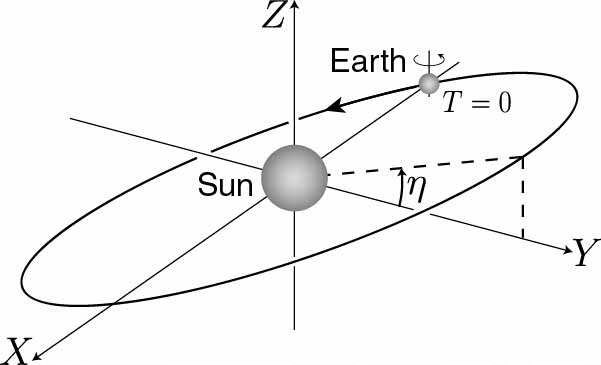
\includegraphics[scale=0.22]{SCF.png}
       	\end{center}
    \end{figure}
\end{minipage}%
\begin{minipage}{0.5\textwidth}
    \begin{itemize}[label=$\triangleright$]
        \item Axe $Z$ : colinéaire à l'axe de rotation de la Terre.
        \item Axe $X$ : pointe vers le point vernal d'équinoxe (voir \figurename{\ref{vernalequinox}}).
        \item Axe $Y$ : complète la base directe. Le plan $XY$ est donc co-planaire au plan équatorial.
    \end{itemize}
\end{minipage}%

\vspace{0.5cm}

    Les points vernaux sont les points d'intersection entre deux plans : le plan écliptique (plan de révolution) et le plan équatorial (plan de rotation de la Terre sur elle-même). 
    
    Au cours de son mouvement, le Soleil croise les points vernaux, l'un en passant de l'hémisphère Nord à l'hémisphère Sud (nœud descendant) l'autre en passant de l'hémisphère Sud à l'hémisphère Nord (nœud ascendant). On nomme point vernal d'équinoxe (parfois appelé \emph{point d'équinoxe de printemps} ou encore \emph{point $\gamma$}) le nœud ascendant.
    \begin{figure}[H]
        \begin{center}
            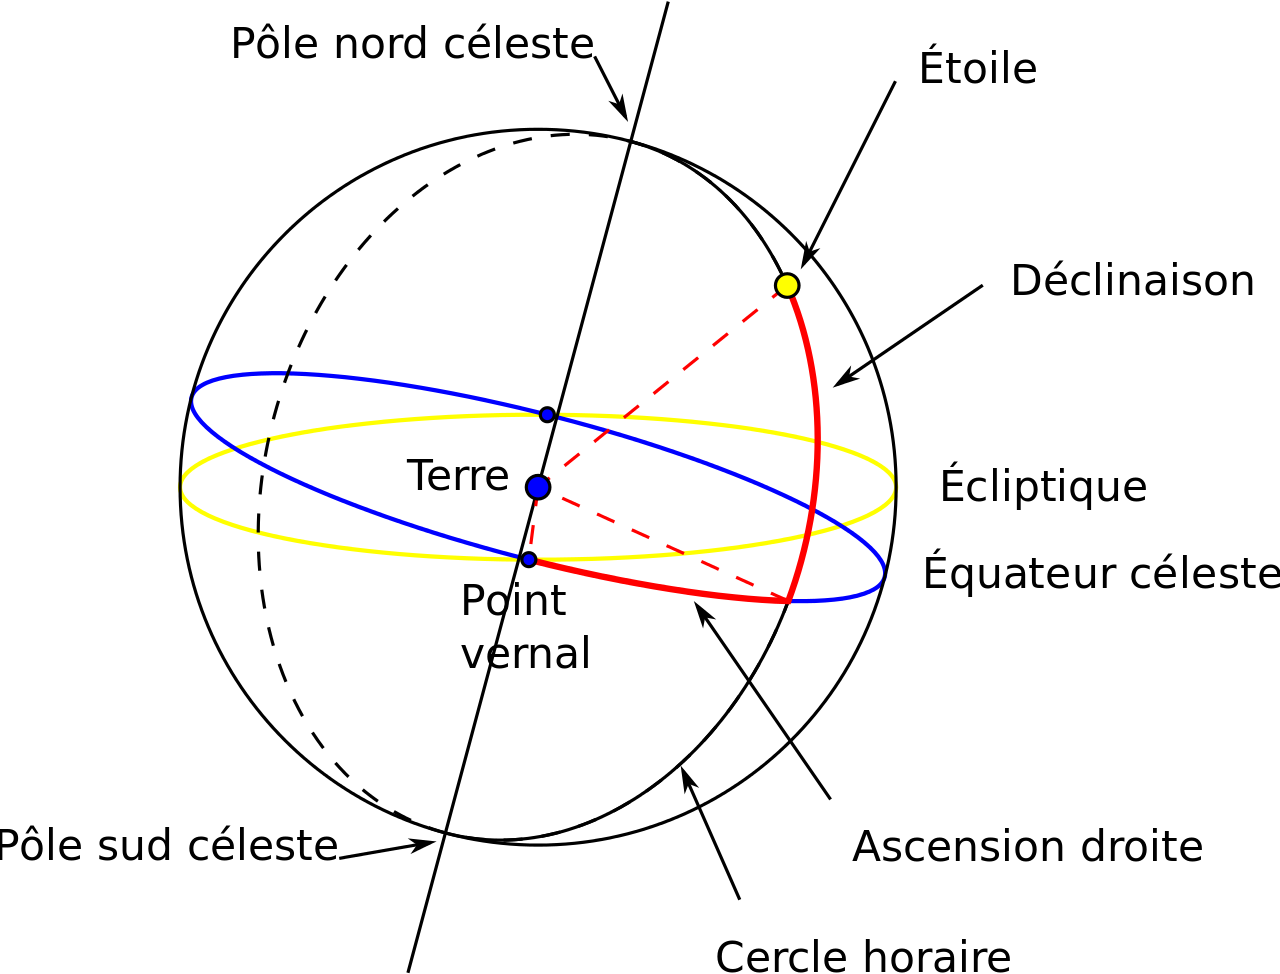
\includegraphics[scale=0.2]{pointVernal.png}
            \caption{Point Vernal quand le soleil passe de l'hémisphère Sud au Nord}
            \label{vernalequinox}
        \end{center}
    \end{figure}
    En raison de la précession des équinoxes (effet gravitationnel) et de la nutation (effet géométrique dû au fait que l'orbite terrestre  n'est pas circulaire mais ellipsoïdale) de la Terre, le point vernal oscille et revient à sa position en 260 siècles. En raison de ce mouvement, on considère comme référence les coordonnées du point vernal au 1er Janvier 2000 à midi UTC (date nommée J2000).
\newline    

 Pour passer du SCF au référentiel de la Terre il faut prendre en compte les trois transformations de Lorentz suivantes :
\begin{description}
    \item [Le boost orbital de la Terre]
    \begin{sloppypar}
        La Terre possède une vitesse orbitale moyenne $v_\oplus \sim \SI{29,783}{\kilo\m\per\s}$ ou de manière relativiste $\beta_\oplus \approx \SI{1e-4}{}$. Au LHC à \SI{13}{\TeV}, les quarks top auront un facteur relativiste en moyenne de $\beta_{\Ptop} = \num{0.76490}$ (voir \tablename{\ref{tab:vitesse_top}}). En utilisant la relation de combinaison des vitesses relativiste, valable tangentiellement, on a :
        \begin{equation}
            \beta_{\Ptop + \oplus} = \frac{\beta_{\Ptop} + \beta_\oplus}{1 + \beta_{\Ptop} \beta_\oplus} = \frac{ \num{e-4}+ \num{0.76490}}{1 + \num{0.76490e-4}} = \num{0.76494} \approx \beta_{\Ptop}
        \end{equation}
        Le boost de la Terre est négligeable devant celui des quarks top créés au LHC.
    \end{sloppypar}
    \item [La révolution de la Terre]
    \begin{sloppypar}
    La révolution de la Terre s'étale sur un an. Ainsi les effets de cette rotation sont très ténus. De plus le LHC n'est pas actif continûment sur une année entière. La sous-activité hivernale, par exemple, introduit des biais statistiques importants.
    \end{sloppypar}
    \item [La rotation de la Terre sur elle-même]
    \begin{sloppypar}
    Journalière, elle est la transformation de Lorentz qui va le plus intensément influer sur l'impulsion des quarks top en jeu.
    \end{sloppypar}
\end{description}

\begin{table}
\begin{center}
\begin{tabular}{c| cc}
    \noalign{\smallskip}\hline\noalign{\smallskip}
    $\sqrt{s}$ de la collision & Vitesse en \si{\GeV\per\c} &$\beta$ \\
    \noalign{\smallskip}
    \hline \hline
    \noalign{\smallskip}
    \SI{13}{\TeV}& \num{401.299}   & \num{0.76490} \\
    \SI{14}{\TeV}& \num{415.371}   & \num{0.79173} \\
    \SI{27}{\TeV}& \num{572.736}   & \num{0.82642} \\
    \SI{100}{\TeV}& \num{1128.42}  & \num{0.89163} \\
    \noalign{\smallskip}\hline\noalign{\smallskip}
\end{tabular}
\caption{Vitesse moyenne d'un quark top généré dans une collision \Pproton-\Pproton pour différentes valeurs d'énergies $\sqrt{s}$ au centre-de-masse, avec une erreur \SI{\sim 1}{‰}.}
\label{tab:vitesse_top}
\end{center}
\end{table}


Parmi ces trois transformations, seule la rotation de la Terre sur elle-même n'est pas négligeable. La rotation dépendante d'un paramètre temporel $t$ a pour incidence une transformation des tenseurs $A^{\mu\nu}$ :
\begin{equation}
    A^{\alpha \beta}_\odot \rightarrow R^\mu_\alpha(t) R^\nu_\beta(t) A^{\alpha \beta}_\oplus
\end{equation}
où $\odot$ représente le SCF, $\oplus$ un référentiel terrestre et les $R^\mu_\alpha$ sont les rotations du référentiel de la Terre vers le SCF. En vertu de la violation de la symétrie de Lorentz les lois physiques vont répondre aux équations suivantes :
\begin{align}
    \sigma_\mathrm{SME} &= \left( 1 +  (c_L)_{\mu\nu} R^\mu_\alpha(t) R^\nu_\beta(t) A^{\alpha \beta}_{L\oplus} +  (c_R)_{\mu\nu}  R^\mu_\alpha(t) R^\nu_\beta(t) A^{\alpha \beta}_{R\oplus} \right) \sigma_\mathrm{SM} \\
   \sigma_\mathrm{SME} &= \left( 1 +  c_{\mu\nu} R^\mu_\alpha(t) R^\nu_\beta(t) A^{\alpha \beta}_{C\oplus} + d_{\mu\nu}  R^\mu_\alpha(t) R^\nu_\beta(t) A^{\alpha \beta}_{D\oplus} \right) \sigma_\mathrm{SM}
\end{align}

\section{Référentiel de l'expérience CMS}
L'étude physique se fera dans le cadre de l'expérience CMS dont une présentation sera faite au chapitre suivant. Pour construire notre modèle phénoménologique, il nous faut donc définir le référentiel de CMS puis établir la transformation de référentiels. Le référentiel de CMS est introduit plus précisément dans le paragraphe \ref{chap3:CMS}. 


La base CMS $ \left\{ x,y,z \right\} $ est définie par \cite{CMSExperiment}

\begin{minipage}{0.5\textwidth}
    \begin{figure}[H]
       	\begin{center}
            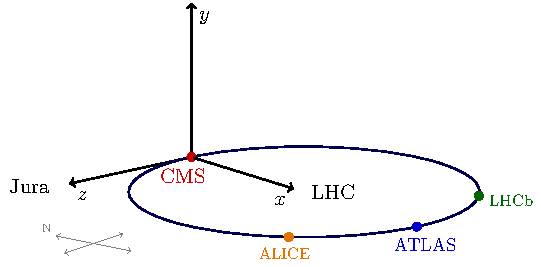
\includegraphics[scale=0.6]{tikz0.pdf}
       	\end{center}
    \end{figure}
\end{minipage}%
\begin{minipage}{0.5\textwidth}
    \begin{itemize}[label=$\triangleright$]
        \item Axe $x$ : pointe vers le centre de l'anneau du LHC.
        \item Axe $z$ : tangent au LHC avec un sens trigonométrique.
        \item Axe $y$ : normal au plan du LHC.
    \end{itemize}
\end{minipage}%

\subsection{Changement de mesure temporelle}

    Plusieurs définitions ont cours. Il est donc impératif de faire un lien entre le temps sidéral (temps GMST), pratique pour l'étude des évènements astronomiques comme la rotation de la Terre sur elle-même, et le temps Unix (temps UTC) qui est le temps utilisé par la collaboration CMS.
    
    \begin{description}
    \item[Temps Atomique international (SI)] 
    \begin{sloppypar}
        Il s'agit de la définition de la seconde du Système International d'unités. Le Bureau International des Poids et Mesures la définit en 1967 comme "la durée de 9 192 631 770 périodes de la radiation correspondant à la transition entre les deux niveaux hyperfins de l'état fondamental de l'atome de césium 133". 
    \end{sloppypar}
    \item[Temps Universel Solaire (UT1)] 
    \begin{sloppypar}
        Le temps solaire est basé sur le croisement moyen du Soleil avec le méridien de Greenwich à 12h. Sa définition est nécessaire pour comprendre la definition du temps Unix (UTC). La moyenne est utilisée car la durée du jour solaire varie périodiquement à cause de l'excentricité de l'orbite de la terre.
        On définit ainsi la seconde par le biais de la période solaire $T_\mathrm{sol}$ :
        \begin{equation}
            T_\mathrm{sol} = \SI{86400}{\s(UT1)} \sim \SI{86400.002}{\s(SI)}
        \end{equation} 
    \end{sloppypar}
    \item[Temps Universel coordonné (UTC)] 
    \begin{sloppypar}
        Il s'agit d'un temps civil et également le temps fourni par le GPS du LHC sous forme de temps informatique ou temps Unix. Il est basé sur le temps atomique pour assurer une stabilité et l'exactitude. Cependant, il a pour but d'être relié à la rotation de la Terre UT1. L'idée ici est de définir un temps qui diffère du temps SI d'un nombre entier de secondes. Par défaut les jours sont définis par \SI{86400}{\s(SI)} mais de plus on maintient 
        \begin{equation}
            \left| \mathrm{UTC} - \mathrm{UT1} \right| < \SI{0.9}{\s}
        \end{equation}  
        en ajoutant aussi souvent qu'il le faut des "secondes intermédiaires"\cite{McCarthy_2008}. La distribution de ces secondes est présentée dans la figure \figurename{\ref{DUT1}}.
        Le temps UNIX a pour origine le 1er Janvier 1970 minuit UTC. Cette origine se nomme l'\emph{UNIX epoch}.
        \begin{figure}
        \begin{center}
            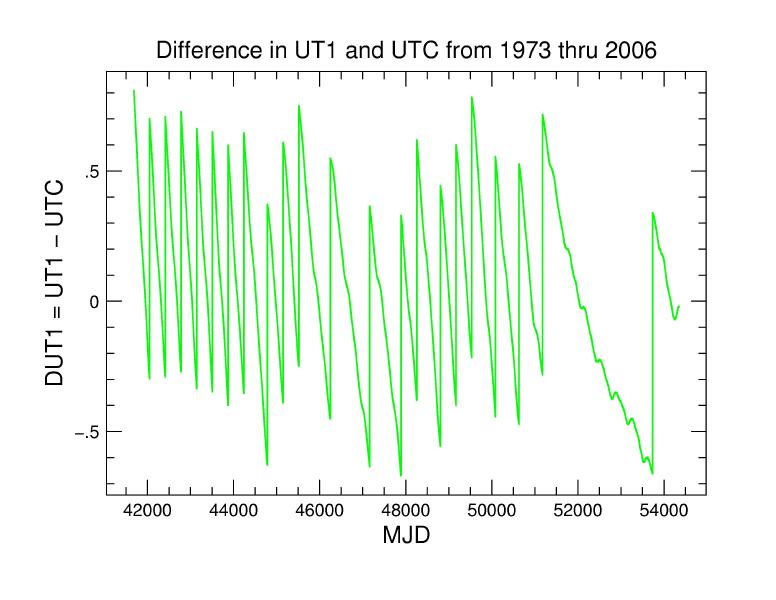
\includegraphics[scale=0.4]{DUT1.jpg}
            \caption{Data Source: IERS Rapid Service/Prediction Center. MDJ correspond au Jour Julien Modifié, jour exprimé en temps sidéral (voir \ref{sideraltime}) avec origine au 17 novembre 1858 à minuit.}
            \label{DUT1}
        \end{center}
        \end{figure} 
    \end{sloppypar}
    \item[Temps Sidéral au Méridien de Greenwich (GMST)] \label{sideraltime}
    \begin{sloppypar}
        On définit le jour sidéral comme le temps qu'il faudra à un astre donné (conventionnellement un quasar lointain) pour revenir à sa position dans le ciel observée depuis la Terre. Formellement le temps GMST et le temps UT1 sont obtenus par une transformation linéaire fixe \cite{Aoki} utilisant une grandeur temporelle intermédiaire nommée jour Julien.
        \begin{equation}
            T_\mathrm{sid} = \SI{86400}{\s(GMST)} = \SI{86164.0989}{\s(UT1)} = \SI{ 86164.1009}{\s(UTC)}
        \end{equation} 
    \end{sloppypar}
    \end{description}

\begin{table}[H]
    \begin{center}
        \begin{tabular}{c|cc}
            \noalign{\smallskip}\hline\noalign{\smallskip}
             & Date & Jour Julien \cite{Aoki} \\
            \noalign{\smallskip}
            \hline \hline
            \noalign{\smallskip}
            J2000 Epoch & 1 Janvier 2000, 12:00:00 UT1 & JD \SI{2451545.0}{UT1}\\
            Unix Epoch & 1 Janvier 1970, 00:00:00 UTC & JD \SI{2440587.5}{UTC}\\
            \noalign{\smallskip}\hline\noalign{\smallskip}
        \end{tabular}
        \caption{Résumé de différents temps initiaux conventionnels.}
    \end{center}
\end{table}


    L'idée, ici, est que le choix du SCF comme référentiel privilégie l'utilisation du temps sidéral (avec J2000 comme origine) pour l'étude de la rotation de la Terre. Mais CMS va nous donner des temps type UTC (Unix). Pour passer de l'un à l'autre, on opère une transformation affine \cite{Aoki} :
    \begin{equation}
        \Omega_\mathrm{GMST} t_\mathrm{SCF} = \Omega_\mathrm{UTC} t_\mathrm{CMS} + \phi 
    \end{equation}
    avec $\phi$ une phase et : 
    \begin{align}
            \Omega_\mathrm{GMST} &= \frac{2\pi}{T_\mathrm{sid}\mathrm{(GMST)}} &= \frac{2\pi}{86400} &= \SI{7.2722e-5}{\si{\rads}(GMST)}\\
            \Omega_\mathrm{UTC} &= \frac{2\pi}{T_\mathrm{sid}\mathrm{(SI)}} &= \frac{2\pi}{86164}  &=  \SI{7.2921e-5}{\rads(SI)}
    \end{align}

    Il faut maintenant calculer la valeur de la phase. Il s'agit de l'angle provenant  du passage de l'origine UNIX epoch à J2000 ($\phi_{\mathrm{UNIX}\rightarrow\mathrm{J2000}}$) mais également d'une longitude effective $\phi_\mathrm{(long)}$ décrite dans le paragraphe suivant. 
    
    Cela revient à connaître la position du méridien de Greenwich à l'UNIX epoch. Le calcul a déjà été fait pour nous \cite{Aoki} et cette transformation vaut : 
    \begin{equation}
        t_{\mathrm{UNIX}\rightarrow\mathrm{J2000}} = \SI{24055 \pm 6}{\s(GMST)}
    \end{equation}
    ce qui donne : 
    \begin{equation}
        \phi_{\mathrm{UNIX}\rightarrow\mathrm{J2000}} = \Omega t_{\mathrm{UNIX}\rightarrow\mathrm{J2000}} =   \SI{1.7493}{\radian} = \SI{100.23}{\degree}
    \end{equation}
    
    La longitude effective $\phi_\mathrm{(long)}$ est définie comme l'angle entre le faisceau de protons et le méridien de Greenwich. Une représentation graphique de cet angle est présentée dans la figure \figurename{\ref{effectivelong}}.
      	\begin{figure}
      		\begin{center}
      			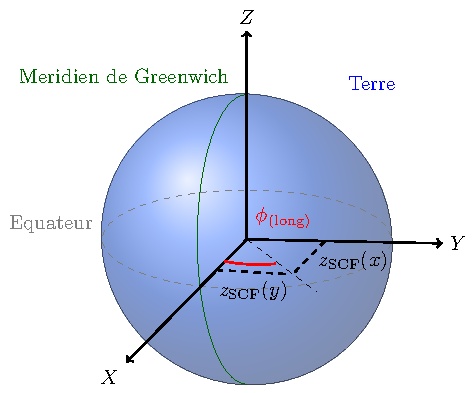
\includegraphics[width=0.6\textwidth]{effectivelong.pdf}
      			\caption{Schéma de la longitude effective.}
                  \label{effectivelong}
      		\end{center}
      	\end{figure}
     
    Pour trouver cette longitude effective, on applique la matrice de rotation SCF$\rightarrow$CMS (voir section suivante) sur l'axe du faisceau de particules du LHC $z_\mathrm{CMS} = (0,0,1)$ afin d'avoir l'expression de ce dernier dans le SCF :
    \begin{equation}
     z_\mathrm{SCF} = R z_\mathrm{CMS}
    \end{equation}
    Puis, grâce à une application trigonométrique, on obtient : 
        \begin{equation}
            \phi_\mathrm{long} = \arctan{ \left( \frac{z_\mathrm{SCF}(x)}{z_\mathrm{SCF}(y)} \right)} = \SI{1.5336}{\radian} = \SI{87.8705}{\degree}
        \end{equation}



    \begin{equation}\boxed{
        \Omega_\mathrm{GMST} t_\mathrm{sideral} = \Omega_\mathrm{UT1/UTC} (t_\mathrm{CMS}) +  \phi_\mathrm{Unix} +  \phi_\mathrm{long}} 
    \end{equation}

    En temps Unix, les valeurs peuvent vite devenir extrêmement élevées. Il est donc très commode de définir un temps $t_0$ plus avancé (le 1er Janvier de l'année de la prise de données par exemple) pour alléger les valeurs numériques. Ces valeurs $t_0$ sont présentées dans le tableau \tablename{\ref{t0value}}.

    \begin{table}
        \begin{center}
            \begin{tabular}{ccc}
                \noalign{\smallskip}\hline\noalign{\smallskip}
                 Date & Horaire & Temps Unix (\SI{}{\second (UTC)})\\
                \noalign{\smallskip}
                \hline \hline
                \noalign{\smallskip}
                01-01-2016& $00:00:00$ & 1451606400 \\
                01-01-2017& $00:00:00$ & 1483228800\\
                01-01-2018& $00:00:00$ & 1514764800 \\
                \noalign{\smallskip}\hline\noalign{\smallskip}
            \end{tabular}
            \caption{Valeur des $t_0$ fixés au 1er Janvier Minuit de chaque année de prise de données du Run II du LHC.}
            \label{t0value}
        \end{center}
    \end{table}
     
    En guise d'application numérique, on déduit pour l'année 2017 que le temps sidéral est donné par :
    \begin{align*}
        t_\mathrm{sideral} &= \frac{\Omega_\mathrm{UT1}(t_\mathrm{CMS} - t_0 ) +  \phi_\mathrm{Unix} +  \phi_\mathrm{long} }{\Omega_\mathrm{GMST}} \\
        &= \frac{ \SI{7.2921e-5}{\rads(UT1)} \times  (t_\mathrm{CMS} - \SI{1483228800}) + \SI{3.2830}{\radian}}{\SI{7.2722e-5}{\rads(GMST)}}
    \end{align*}



\subsection{Rotation SCF $\rightarrow$ CMS}

        Pour caractériser la rotation de la terre sur elle-même il faut faire appel à deux angles en plus de la vitesse angulaire de la Terre.
        Le premier angle est la \underline{latitude} $\lambda$, vieille coordonnée marine qui commence à l'équateur ($\lambda = $ \SI{0}{\degree}) et qui finit aux pôles ($\lambda = $ \SI{\pm 90}{\degree}).
        Le deuxième angle est l'azimut $\theta$ au LHC \cite{Jones}. L'azimut mesure l'angle entre un vecteur tangent à l'anneau (dans le sens horaire) et le vecteur colinéaire au méridien de Greenwich (orienté Nord).
    	\begin{figure}[H]
    		\begin{center}
    			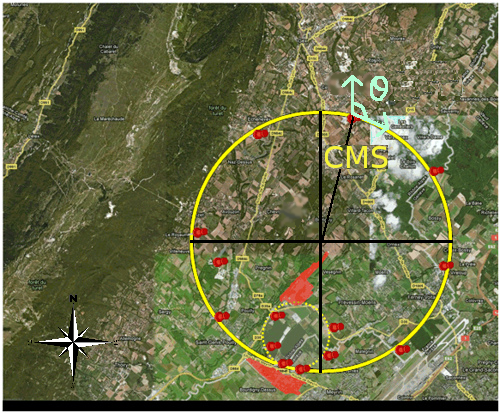
\includegraphics[scale=0.5]{cernLHCgoogleAngle.png}
    			\caption{Image Google Earth de l'anneau du LHC}
    		\end{center}
    	\end{figure}
        Un résumé des angles est montré dans le tableau \tablename{\ref{anglesderotation}}.
    \begin{table}
        \begin{center}
            \begin{tabular}{c|ccc}
                \noalign{\smallskip}\hline\noalign{\smallskip}
                 Angle & Variable & radian (\si{\radian}) &  degrés (\si{\degree}) \\
                \noalign{\smallskip}
                \hline \hline
                \noalign{\smallskip}
                Azimut & $\theta$ & \SI{1.7677 \pm 0.0001}{} & \SI{101.2790 \pm 0.0001}{}\\
                Latitude & $\lambda$ & \SI{ 0.8082 \pm 0.0001}{} & \SI{ 46.309 \pm 0.003}{}\\
                Longitude & $\ell$ &  \SI{0.1061 \pm 0.0001}{} &  \SI{6.0766 \pm 0.0001}{}\\
                \noalign{\smallskip}\hline\noalign{\smallskip}
            \end{tabular}
            \caption{Angles paramètres de la matrice de changement de base \cite{Jones}.}
            \label{anglesderotation}
        \end{center}
    \end{table}

        On rappelle que le but est de passer par rotation du référentiel SCF au référentiel de CMS.
        La première étape est de définir une base au point 5 du LHC (CMS). Par convention, on a l'axe $z$ suivant le faisceau dans le sens des aiguilles d'une montre et l'axe $x$ perpendiculaire à $z$ pointant vers le centre de l'anneau. On construit ensuite notre axe $y$ qui pointe vers la surface de sorte à obtenir un repère orthonormé direct.
        La seconde étape est de construire la matrice de rotation $R$ dépendante du temps qui nous permet la transition entre le SCF et le référentiel de CMS :
        \begin{equation*}
            \mathcal{B}_\mathrm{CMS}(x,y,z) \overset{R(t)}{\longrightarrow} \mathcal{B}_\mathrm{SCF}(X,Y,Z)
        \end{equation*}
        où $\mathcal{B}$ représente les bases des référentiels.
        Dans la suite, toutes les rotations seront dans le \underline{sens trigonométrique}.

\subsubsection{Matrices de rotation}

\begin{description}
\item[Première rotation $R_z\left(\frac{\pi}{2}\right)$.] 
\begin{sloppypar}
    C'est une rotation autour de l'axe $z$ qui rend l'axe $x$ normal au plan du LHC. Cela permet d'avoir l'axe $x$ normal au plan tangent de la Terre, à la localisation du LHC. La nouvelle base est donnée par $\mathcal{B}_\mathrm{CMS}(x',y',z)$.
    \begin{minipage}{0.5\textwidth}
        \begin{equation*}\footnotesize
            R_z\left(\frac{\pi}{2}\right) =
            \begin{pmatrix}
                1 & 0 & 0 & 0 \\
                0 & 0 & -1 & 0 \\
                0 & 1 & 0 & 0 \\
                0 & 0 & 0 & 1
            \end{pmatrix}
        \end{equation*}
    \end{minipage}%
    \begin{minipage}{0.5\textwidth}
        \begin{figure}[H]
            \begin{center}
                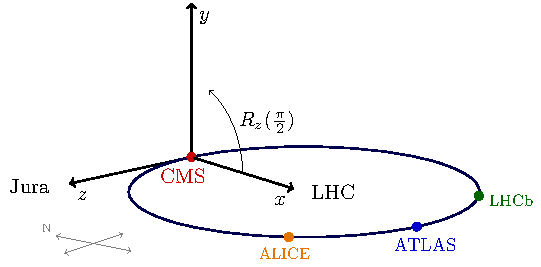
\includegraphics[scale=0.6]{tikz2.pdf}
            \end{center}
        \end{figure}
    \end{minipage}%
\end{sloppypar}
\item[Deuxième rotation $R_{x'}\left(\pi - \theta)\right)$.] 
\begin{sloppypar}
On veut orienter l'axe $z$ en direction du Nord. On tourne dans le sens trigonométrique autour de l'axe $x'$ avec un angle $\pi - \theta$ (co-azimut).
 La nouvelle base est donnée par $\mathcal{B}_\mathrm{CMS}(x',y'',z'')$.
\begin{minipage}{0.5\textwidth}
    \begin{equation*}\footnotesize
        R_{x'}\left(-(\pi - \theta)\right)
        =
        \begin{pmatrix}
            1 & 0 & 0 & 0 \\
            0 & 1 & 0 & 0 \\
            0 & 0 & -\cos(\theta) & \sin(\theta) \\
            0 & 0 & -\sin(\theta) & -\cos(\theta)
        \end{pmatrix}
    \end{equation*}
\end{minipage}%
\begin{minipage}{0.5\textwidth}
    \begin{figure}[H]
        \begin{center}
            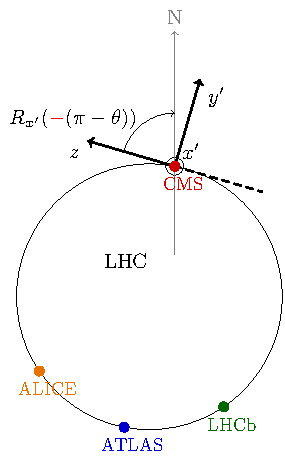
\includegraphics[scale=0.6]{tikz3.pdf}
        \end{center}
    \end{figure}
\end{minipage}%
\end{sloppypar}
\item[Troisième rotation $R_{y''}\left(\lambda\right)$.] 
\begin{sloppypar}
Rotation autour de l'axe $y''$ pour faire coïncider l'axe $z$ avec l'axe $Z$ du SCF.  La nouvelle base est donnée par $\mathcal{B}_\mathrm{CMS}(x'',y'',Z)$.
\begin{minipage}{0.5\textwidth}
    \begin{equation*}\footnotesize
        R_{y''}\left(\lambda\right) =
        \begin{pmatrix}
            1 & 0 & 0 & 0 \\
            0 & \cos(\lambda) & 0 & \sin(\lambda) \\
            0 & 0 & 1 & 0 \\
            0 & -\sin(\lambda) & 0 & \cos(\lambda)
        \end{pmatrix}
    \end{equation*}
\end{minipage}%
\begin{minipage}{0.5\textwidth}
    \begin{figure}[H]
    \begin{center}
        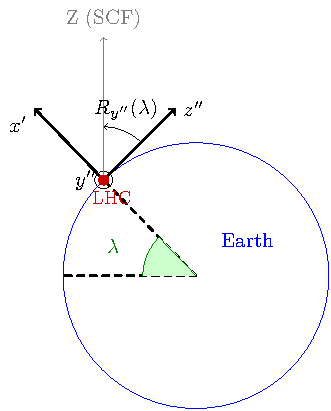
\includegraphics[scale=0.6]{tikz4.pdf}
    \end{center}
    \end{figure}
\end{minipage}%
\end{sloppypar}
\item[Quatrième rotation $R_Z\left(\Omega t\right)$.] 
\begin{sloppypar}
Une dernière rotation autour de l'axe $Z$ a deux buts : suivre la rotation de la Terre au cours du temps et se synchroniser avec le SCF : $\left\{ x'', y''\right\} \Rightarrow \left\{ X, Y\right\}$.
\begin{equation*}\footnotesize
    R_Z\left(\Omega t\right) =
    \begin{pmatrix}
        1 & 0 & 0 & 0 \\
        0 & \cos(\Omega t) & -\sin(\Omega t) & 0 \\
        0 & \sin(\Omega t) & \cos(\Omega t) & 0 \\
        0 & 0 & 0 & 1
    \end{pmatrix}
\end{equation*}
Avec $\Omega t =\Omega_\mathrm{UTC} t_\mathrm{CMS} + \phi_\mathrm{Unix} +  \phi_\mathrm{longitude} $ 
\end{sloppypar}
\end{description}

%\def\sl{\sin{\lambda}}%
%\def\cl{\cos{\lambda}}%
%\def\st{\sin{\theta}}%
%\def\ct{\cos{\theta}}%
\def\sl{\mathrm{s}_\lambda}%
\def\cl{\mathrm{c}_\lambda}%
\def\st{\mathrm{s}_\theta}%
\def\ct{\mathrm{c}_\theta}%

\subsubsection*{La matrice de rotation SCF$\rightarrow$CMS}
En résumé : 
\begin{equation}
    R\left(\lambda,\theta\right) = R_{y''}\left(\lambda\right) R_{x'}\left(-(\pi - \theta)\right) R_z\left(\frac{\pi}{2}\right) R_Z\left(\Omega t\right)
\end{equation}

\begin{equation}\footnotesize \label{rotation}
    R(\lambda,\theta,t) =
    \begin{pmatrix}
        1 & 0 & 0 & 0 \\
        0 & -\cos(\Omega t)\sl\ct + \sin(\Omega t)\ct & -\cos(\Omega t)\cl &  -\cos(\Omega t)\sl\ct - \sin(\Omega t)\st \\
        0 & -\sin(\Omega t)\sl\ct - \cos(\Omega t)\ct & -\sin(\Omega t)\cl  & -\sin(\Omega t)\sl\ct + \cos(\Omega t)\st \\
        0 & -\cl\st & -\sl & -\cl\ct
    \end{pmatrix}
\end{equation}

\subsection{Les quantités $A^{\mu\nu}$}

Pour calculer les quantités $A^{\mu\nu}$ introduites dans \eqref{amunu}, dans le référentiel de CMS, des simulations pour le processus $\ttbar \rightarrow \Pbottom \Pleptonplus \Pnulepton +  \APbottom \Pleptonminus \APnulepton$ ont été réalisées en générant des évènements au niveau partonique avec \texttt{MadGraph\_aMC@NLO} \cite{Madgraph} au premier ordre avec le PDF NNPDF2.3 LO \cite{PDF} dans le Modèle Standard.

\begin{table}[H]
\begin{center}
    \begin{tabular}{c|cc}
    \noalign{\smallskip}\hline\noalign{\smallskip}
    Énergie au centre & Nombres & Type de   \\
    de masse & d'évènements & collisions  \\
    \noalign{\smallskip}
    \hline \hline
    \noalign{\smallskip}
    \SI{13}{\TeV} & \SI{5e-6}{}&\Pproton{}-\Pproton{}  \\
    \noalign{\smallskip}\hline\noalign{\smallskip}
    \end{tabular}
\end{center}
\end{table}
Les moyennes $\langle A^{\mu \nu}\rangle$ sont obtenues par moyenne arithmétique des $A^{\mu\nu}$ de chaque évènement. La pertinence de ce choix est expliquée en annexe \ref{B:averageamunu}.
  
Les $A^{\mu\nu}$ sont générées de manières différentes pour la production par annihilation quark/antiquark et pour la fusion de gluon \cite{KosteleckyPheno}. Il est alors impératif de pondérer la valeur des  $A^{\mu\nu}$ par leur ratio de production (noté ici $\Gamma$) simplement obtenu par le rapport du nombre d'évènements par mode de production sur le nombre d'évènements total. Ces ratios dépendent de l'énergie au centre de masse des réactions engendrant les productions.
On peut voir dans la figure \figurename{\ref{fig:amunu}} quelques exemples d'histogrammes de la valeur des différentes composantes d'un matrice $A^{\mu\nu}$ où pour chaque coefficient de Lorentz $\mu$ et $\nu$ on a la convention $0 \equiv \mathrm{T}$, $1 \equiv \mathrm{X}$, $2 \equiv \mathrm{Y}$ et $3 \equiv \mathrm{Z}$. La totalité des histogrammes présentant les $\langle A^{\mu \nu} \rangle$ de chaque évènement peut être trouvée en annexe \ref{B:amunu}.
\begin{figure}[h]
    \centering
    \subcaptionbox{\label{fig:ZZ}}[0.32\textwidth]{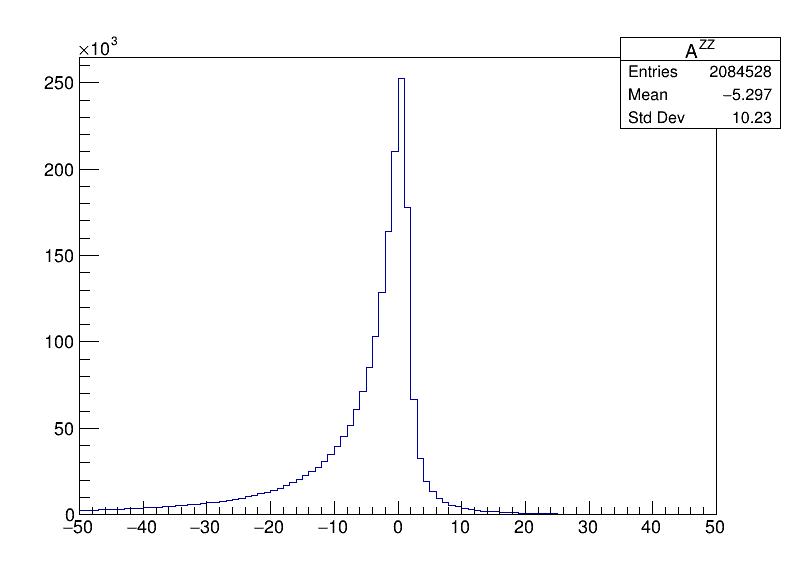
\includegraphics[width=0.32\textwidth]{AZZ.png}} \hfill
    \subcaptionbox{\label{fig:XX}}[0.32\textwidth]{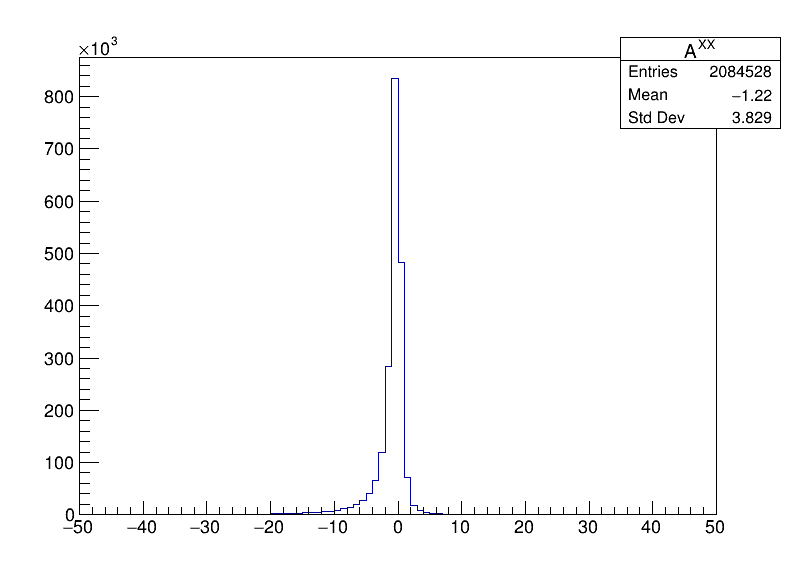
\includegraphics[width=0.32\textwidth]{AXX.png}}
    \subcaptionbox{\label{fig:XY}}[0.32\textwidth]{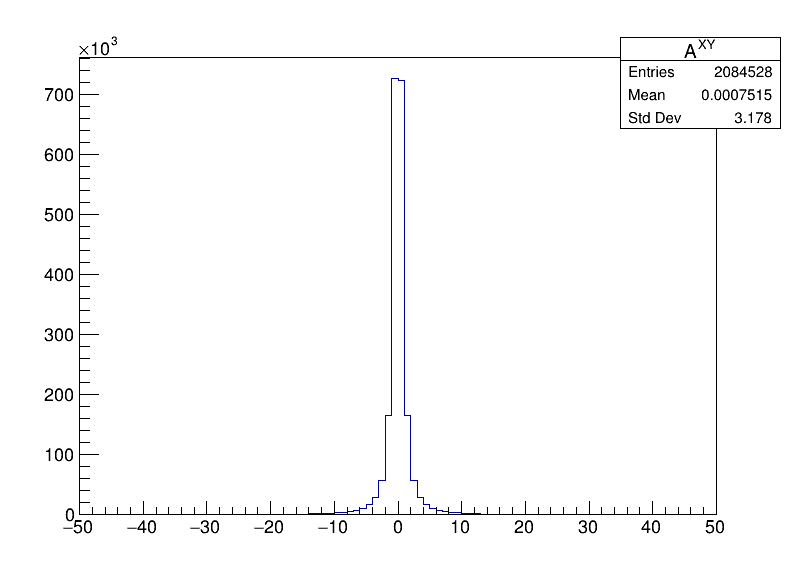
\includegraphics[width=0.32\textwidth]{AXY.png}}
    \caption{Histogramme de valeur des composantes de la matrice $  A^{\mu\nu}_\mathrm{TOT} =  \frac{\Gamma_{\Pquark{}\APquark{}}}{2}  A^{\mu\nu}_{\Pquark{}\APquark{}} + \frac{\Gamma_{\Pgluon{}\Pgluon{}}}{2}  A^{\mu\nu}_{\Pgluon{}\Pgluon{}}+  A^{\mu\nu}_{F} $  pour $\mu\nu =$ ZZ (\subref{fig:ZZ}), XX (\subref{fig:XX}) et XY (\subref{fig:XY}).}
    \label{fig:amunu}
\end{figure}


Au LHC à \SI{13}{\TeV} :
\begin{equation}
    \langle A^{\mu \nu}_{P_{\Pquark{}\APquark{}}} \rangle =
    \begin{pmatrix}
        1.178 \pm 0.007 & 0.000 \pm 0.001 & 0.000 \pm 0.001 & 0.004 \pm  0.008\\
        0.000 \pm 0.001 & 0.195 \pm 0.001 & 0.000 \pm 0.001 & 0.000 \pm  0.001\\
        0.000 \pm 0.001 & 0.000 \pm 0.001 & 0.195 \pm 0.001 & 0.000 \pm  0.001\\
        0.004 \pm 0.008 & 0.000 \pm 0.001 & 0.000 \pm 0.001 & 2.890 \pm 0.007
    \end{pmatrix}
\end{equation}
avec $\Gamma_{\Pquark{}\APquark{}} = 0.114$
\begin{equation}
    \langle A^{\mu \nu}_{P_{\Pgluon{}\Pgluon{}}} \rangle =
    \begin{pmatrix}
        13.55 \pm 0.02& 0.000 \pm 0.001& 0.000 \pm 0.001& 0.00 \pm  0.02\\
        0.000  \pm 0.001& 0.144 \pm 0.001& 0.000 \pm 0.001& 0.000 \pm 0.001 \\
        0.000  \pm 0.001& 0.000 \pm 0.001& 0.143 \pm 0.001& 0.000 \pm 0.001 \\
        0.00  \pm 0.02& 0.000 \pm 0.001& 0.000 \pm 0.001 & 9.42 \pm 0.02
    \end{pmatrix}
\end{equation}
avec $\Gamma_{\Pgluon{}\Pgluon{}} = 0.886$
\begin{equation}
    \langle A^{\mu \nu}_{F} \rangle =
    \begin{pmatrix}
        -31.2 \pm 0.3 & 0.04 \pm 0.05 & 0.00 \pm  0.05 & 0.00 \pm 0.3 \\
        0.04 \pm 0.05 & -1.798 \pm 0.02 & 0.00 \pm  0.02& -0.01 \pm 0.04 \\
        0.00 \pm 0.05 & 0.00  \pm 0.02 & -1.81 \pm 0.02 & 0.05 \pm 0.04\\
        0.00 \pm 0.3  & -0.01 \pm 0.04 & 0.05 \pm  0.04& -20.4 \pm 0.2
    \end{pmatrix}
\end{equation}
Les incertitudes calculées sont purement statistiques et représentent l'incertitude sur la moyenne. Par exemple pour un terme $A^{\mu \nu}_{F}$ la déviation standard est donnée par :
\begin{equation}
    \mathrm{sd}\left( A^{\mu \nu}_{F} \right) = \frac{1}{\sqrt{N}}\sqrt{\sum_{i=0}^{N} \frac{ \left(A^{\mu \nu}_{F}\right)^2_i -  \langle A^{\mu \nu}_{F}\rangle^2  }{N^2} }
\end{equation} 

L'examen des valeurs prises par les matrices suggère les hypothèses de travail pour la suite :
\begin{align}\label{hypotheseAmunu}
    \langle &A^\mathrm{XX} \rangle \simeq \langle A^\mathrm{YY} \rangle \\
     \langle &A^{\alpha \beta} \rangle \simeq 0 \qquad \mathrm{pour} \qquad \alpha \neq \beta
\end{align}
Ces hypothèses ont également été faites par l'expérience D$\emptyset$ au Tevatron \cite{D0}.
    \subsubsection{La fonction de modulation}
    
    La modulation de la section efficace au cours du temps est la signature caractéristique de la violation de Lorentz, il est donc nécessaire de construire un objet mathématique qui puisse en rendre compte. Dans un référentiel autre que le SCF on aura: 
    \begin{equation}
        w = 1 + f(t)
    \end{equation}
    
    A l'aide des hypothèses présentées dans \eqref{hypotheseAmunu}, de la matrice de rotation \eqref{rotation} ainsi que des équations \eqref{amunudecomposition}, on construit en prenant $x_{\mu\nu}$ un coefficient de Wilson quelconque :
    \begin{align}
        f(t) &= x_{\mu\nu} R^\mu_\alpha(t) R^\nu_\beta(t) \langle A^{\mu\nu} \rangle \nonumber \\
        &=  x_{\mu\nu} \left(  R^\mu_T(t)  R^\nu_T(t) \langle A^\mathrm{TT} \rangle  +  2R^\mu_X(t)  R^\nu_X(t) \langle A^\mathrm{XX} \rangle +  R^\mu_Z(t)  R^\nu_Z(t) \langle A^\mathrm{ZZ} \rangle \right) \nonumber \\
        &= x_{TT} \langle A^\mathrm{TT} \rangle + x_{ij} \left( 2R^i_X(t)  R^j_X(t) \langle A^\mathrm{XX} \rangle +  R^i_Z(t)  R^j_Z(t) \langle A^\mathrm{ZZ} \rangle \right)
    \end{align}
avec $i,j = X, Y, Z$. On observe ainsi que la contribution temporelle n'est effective que dans le cas de l'absence d'oscillation, ce qui représente une observable difficile à mesurer. En effet, une simple mise à l'échelle constante de la section efficace de production \ttbar pourrait être interprétée comme une incertitude provenant de la QCD.  Sont ainsi exclus de l'analyse tout poids ne générant pas d'oscillation.

Pour rappel, les formes des  $A^{\mu\nu}$ dépendent du coefficient de Wilson qui leur est couplé. Un résumé de ces formes est donné dans la table \tablename{\ref{tab:wilson}}.
\begin{table}
    \begin{center}
        \begin{tabular}{c|ccc}
            \noalign{\smallskip}\hline\noalign{\smallskip}
            & Forme générale &  $\langle A^\mathrm{XX} \rangle$ &  $\langle A^\mathrm{ZZ} \rangle$ \\
            \noalign{\smallskip}
            \hline \hline
            \noalign{\smallskip}
            $c_{L\mu\nu}$ & $\frac{\Gamma_{\Pquark{}\APquark{}}}{2}  A^{\mu\nu}_{\Pquark{}\APquark{}} + \frac{\Gamma_{\Pgluon{}\Pgluon{}}}{2}  A^{\mu\nu}_{\Pgluon{}\Pgluon{}}+  A^{\mu\nu}_{F} $ &  \SI{-1.723}{} & \SI{-16.107}{} \\

            $c_{R\mu\nu}$ & $\frac{\Gamma_{\Pquark{}\APquark{}}}{2}  A^{\mu\nu}_{\Pquark{}\APquark{}} + \frac{\Gamma_{\Pgluon{}\Pgluon{}}}{2}  A^{\mu\nu}_{\Pgluon{}\Pgluon{}} $ & \SI{0.075}{}& \SI{4.336}{}  \\
            \noalign{\smallskip}\hline\noalign{\smallskip}

            $c_{\mu\nu}$ & $\Gamma_{\Pquark{}\APquark{}}  A^{\mu\nu}_{\Pquark{}\APquark{}} + \Gamma_{\Pgluon{}\Pgluon{}} A^{\mu\nu}_{\Pgluon{}\Pgluon{}}+  A^{\mu\nu}_{F} $ &\SI{-1.648}{} &\SI{-11.770}{}  \\

            $d_{\mu\nu}$ & $ A^{\mu\nu}_{F} $ & \SI{-1.798}{}& \SI{-20.443}{}  \\
            \noalign{\smallskip}\hline\noalign{\smallskip}
        \end{tabular}
        \caption{Table de valeur des quantités $A^{\mu\nu}$ pour différents coefficients de Wilson}
        \label{tab:wilson}
    \end{center}
\end{table}



    \subsection{Les équations}
    
    Le modèle standard ne provoquant aucune violation de symétrie de Lorentz se doit d'avoir une fonction de modulation $f(t)$ toujours nulle. Ainsi la fonction de modulation sera la signature d'une violation de Lorentz. On doit donc, pour l'analyse future, préparer les équations de $f(t)$.
    
    Au vu de la forme de la fonction de modulation, seuls les coefficients porteurs d'indices spatiaux seront effectifs. 
    A l'observation des propriétés \eqref{traceless} seules les combinaisons de coefficients  suivantes seront testables : 
    \begin{itemize}[label=$\triangleright$]
        \item $c_\mathrm{XX} = -c_\mathrm{YY}$ (trace nulle)
        \item $c_\mathrm{XY} = c_\mathrm{YX}$ (symétrie de $c_{\mu\nu}$)
        \item $c_\mathrm{XZ} = c_\mathrm{ZX}$ (symétrie de $c_{\mu\nu}$)
        \item $c_\mathrm{YZ} = c_\mathrm{ZY}$ (symétrie de $c_{\mu\nu}$)
    \end{itemize}
    Ces hypothèses ont également été testées par l'expérience D$\emptyset$ au Tevatron \cite{D0}.
\subsubsection{Établissement de l'équation de modulation pour $c_\mathrm{XX} = -c_\mathrm{YY}$}
            En considérant que seuls $c_\mathrm{XX} = -c_\mathrm{YY}$ sont non-nuls. On a :
            \begin{align*}
                \frac{f_\mathrm{SME}^\mathrm{(XX)} (t)}{c_\mathrm{XX}} & =  \left( \left(R_X^X R_X^X + R_Y^X R_Y^X \right) \langle A^\mathrm{XX} \rangle  +  R_Z^X R_Z^X \langle A^\mathrm{ZZ} \rangle   \right)
                \\& = \left( (- c_t s_\lambda s_\theta + s_t c_\theta )^2 + (c_t c_\lambda)^2 \right) \langle A^\mathrm{XX} \rangle + (-c_t s_\lambda c_\theta - s_t 	s_\theta )^2 \langle A^\mathrm{ZZ} \rangle
                \\ & = \underbrace{\left( \left( s_\lambda^2 s_\theta^2 + c_\lambda^2 \right) \langle A^\mathrm{XX} \rangle +s_\lambda^2 c_\theta^2 \langle A^\mathrm{ZZ} \rangle \right)}_{a_1} c_t^2 + \underbrace{\left( c_\theta^2 \langle A^\mathrm{XX} \rangle + s_\theta^2 \langle A^\mathrm{ZZ} \rangle  \right)}_{a_2} s_t^2
                \\ & \qquad + 2 s_t c_t \underbrace{s_\lambda c_\theta s_\theta \left(\langle A^\mathrm{ZZ} \rangle  - \langle A^\mathrm{XX} \rangle \right) }_{a_3}
                \\ & = \frac{a_1}{2}\left(\cos(2 \Omega t) +1\right) + \frac{a_2}{2} \left(1 - \cos(2 \Omega t)\right) + a_3 \sin(2 \Omega t)
                \\ & = \left( \frac{a_1 + a_2}{2} \right) + \left(\frac{a_1 - a_2}{2}\right) \cos(2 \Omega t) + a_3 \sin(2\Omega t )
            \end{align*}
            \begin{align*}
                \frac{f_\mathrm{SME}^\mathrm{(YY)} (t)}{c_\mathrm{YY}} & =  \left( \left(R_X^Y R_X^Y + R_Y^Y R_Y^Y \right) \langle A^\mathrm{XX} \rangle  +  R_Z^Y R_Z^Y \langle A^\mathrm{ZZ} \rangle   \right)
                \\& = \left( (- s_t s_\lambda s_\theta - c_t c_\theta )^2 + (s_t c_\lambda)^2 \right) \langle A^\mathrm{XX} \rangle + (- s_t s_\lambda c_\theta + c_t s_\theta)^2 \langle A^\mathrm{ZZ} \rangle
                \\ & = \underbrace{\left( \left( s_\lambda^2 s_\theta^2 + c_\lambda^2 \right) \langle A^\mathrm{XX} \rangle +s_\lambda^2 c_\theta^2 \langle A^\mathrm{ZZ} \rangle \right)}_{a_1} s_t^2 + \underbrace{\left( 	c_\theta^2 \langle A^\mathrm{XX} \rangle + s_\theta^2 \langle A^\mathrm{ZZ} \rangle  \right)}_{a_2} c_t^2
                \\ & \qquad - 2 s_t c_t \underbrace{s_\lambda c_\theta s_\theta \left(\langle A^\mathrm{ZZ} \rangle  - \langle A^\mathrm{XX} \rangle \right) }_{a_3}
                \\ & = \frac{a_1}{2} \left(1 - \cos(2 \Omega t)\right) + \frac{a_2}{2}\left(\cos(2 \Omega t) +1\right) +  a_3 \sin(2 \Omega t)
                \\ & = \left( \frac{a_1 + a_2}{2} \right) - \left(\frac{a_1 - a_2}{2}\right) \cos(2 \Omega t) - a_3 \sin(2\Omega t )
            \end{align*}
            \begin{equation*}
                f_\mathrm{SME}^\mathrm{(XX,YY)} (t) = c_\mathrm{XX}	\frac{f_\mathrm{SME}^\mathrm{(XX)} (t)}{c_\mathrm{XX}} - c_\mathrm{XX} \frac{f_\mathrm{SME}^\mathrm{(YY)} (t)}{c_\mathrm{YY}}
            \end{equation*}
            \begin{equation}
                \boxed{f_\mathrm{SME}^\mathrm{(XX,YY)} (t) = 2 c_\mathrm{XX} \left( \left(\frac{a_1 - a_2}{2}\right) \cos(2 \Omega t) + a_3 \sin(2\Omega t ) \right)}
            \end{equation}

        Les démonstrations des autres fonctions de modulation sont disponibles en annexe \ref{B:f}. 
        
        \subsubsection{Résumé des équations de modulation}
On a finalement :
            \begin{equation}
                \left\{
                    \begin{array}{ll}
                        f_\mathrm{SME}^\mathrm{(XX)} (t) = 2 c_\mathrm{XX} \left( \left(\frac{a_1 - a_2}{2}\right) \cos(2 \Omega t) + a_3 \sin(2\Omega t ) \right)
                        \\ f_\mathrm{SME}^\mathrm{(XY)} (t) = 2 c_\mathrm{XY} \left( \left( \frac{a_1 - a_2}{2} \right)  \sin(2 \Omega t) - a_3 \cos(2 \Omega t)  \right)
                        \\ f_\mathrm{SME}^\mathrm{(ZX)} (t) = 2 c_\mathrm{XZ} \left(a_4 \cos(\Omega t) + a_5 \sin(\Omega t) \right)
                        \\ f_\mathrm{SME}^\mathrm{(YZ)} (t) = 2 c_\mathrm{YZ} \left(a_4 \sin(\Omega t) - a_5 \cos(\Omega t) \right)
                    \end{array}
                \right.
            \end{equation}
            avec
            \begin{equation}
                \left\{
                    \begin{array} {ll}
                        a_1 = \left( s_\lambda^2 s_\theta^2 + c_\lambda^2 \right) \langle A^\mathrm{XX} \rangle +s_\lambda^2 c_\theta^2 \langle A^\mathrm{ZZ} \rangle
                        \\a_2 = \left( c_\theta^2 \langle A^\mathrm{XX} \rangle + s_\theta^2 \langle A^\mathrm{ZZ} \rangle  \right)
                        \\a_3 = s_\lambda c_\theta s_\theta \left(\langle A^\mathrm{ZZ} \rangle  - \langle A^\mathrm{XX} \rangle \right)
                        \\a_4 = c_\lambda s_\lambda c_\theta^2 \left( \langle A^\mathrm{ZZ} \rangle - \langle A^\mathrm{XX} \rangle  \right)
                        \\a_5 = s_\theta c_\lambda c_\theta \left( \langle A^\mathrm{ZZ} \rangle - \langle A^\mathrm{XX}  \rangle \right)
                    \end{array}
                \right.
            \end{equation}
    \subsection{Représentation graphique}
        Rappelant que les formes de $ \langle A_{\mu\nu} \rangle $ sont dépendantes du coefficient de Wilson avec lequel elles sont contractées, on aura quatre fonctions $f(t)$ d'oscillation, une pour chaque coefficient de Wilson. 
        Ici, ne sont présentées que les modulations pour les couples non-nuls de coefficient de Wilson de la matrice $c_{L\mu\nu}$. Les autres sont disponibles en annexe \ref{B:wilson}.
        
            \begin{figure}[H]
                \begin{center}
                    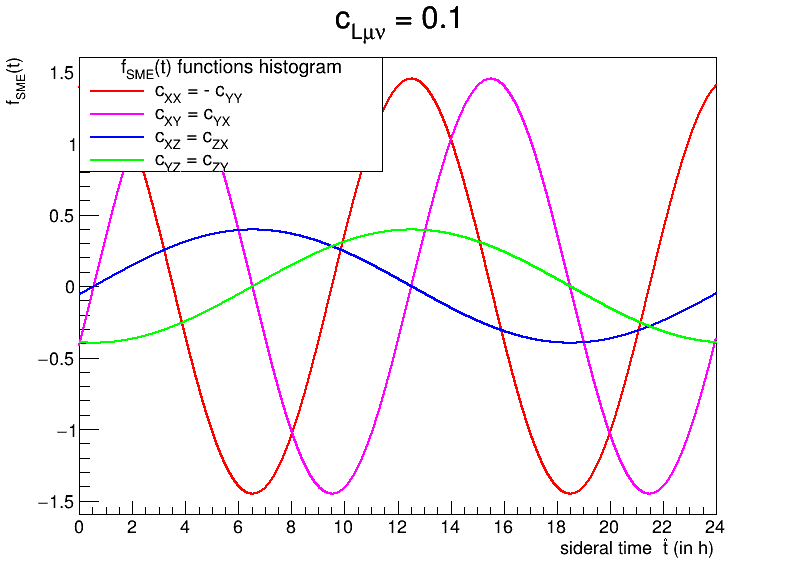
\includegraphics[scale=0.4]{fComparaisonL.png}
                    \caption{Tracé des fonction $f(t)$ pour les différents couples de coefficient gauche non-nuls dans le scenario LHC \SI{13}{\TeV}.}
                \end{center}
            \end{figure}



\section{Sensibilité aux collisionneurs}

Dans cette section est présentée une étude de la précision attendue sur les coefficients de Wilson $c_{\mu\nu}$ dans différents scenarii de collisionneurs. Pour ce faire, les estimations seront faites en premier lieu pour le LHC Run II, puis elles seront extrapolées pour les autres scenarii. 
Les différences fondamentales entre les divers scenarii sont l'énergie au centre de masse $\sqrt{s}$ de l'accélérateur de particules et la luminosité $\mathcal{L}$.
Seront analysés le HL-LHC (High Luminosity LHC) et les hypothétiques HE-LHC (High Energy LHC) et FCC-hh (Futur Circular Collider hadron-hadron) dont les caractéristiques sont résumées dans la table \tablename{\ref{scenarii}}. Les résultats du Tevatron seront également indiqués à titre de comparaison.


\begin{table}
    \begin{center}
        \begin{tabular}{c|ccc}
            \noalign{\smallskip}\hline\noalign{\smallskip}
             Forme générale & $\sqrt{s}$ &  $\mathcal{L}$ & Type de collision\\
            \noalign{\smallskip}
            \hline \hline
            \noalign{\smallskip}
            Tevatron & \SI{1.96}{\TeV}& \SI{5.3}{\per\fb} &\Pproton-\APproton\\
            LHC Run II & \SI{13}{\TeV}& \SI{150}{\per\fb} & \Pproton-\Pproton\\
            HL-LHC & \SI{14}{\TeV}& \SI{3}{\per\ab} & \Pproton-\Pproton \\
            HE-LHC & \SI{27}{\TeV}& \SI{15}{\per\ab} & \Pproton-\Pproton\\
            FCC-hh & \SI{100}{\TeV}& \SI{15}{\per\ab} & \Pproton-\Pproton\\
            \noalign{\smallskip}\hline\noalign{\smallskip}
        \end{tabular}
        \caption{Caractéristiques des différents scenarii.}
        \label{scenarii}
    \end{center}
\end{table}



\subsection{Precision attendue au LHC Run II}

Cette section a pour but d'établir la sensibilité attendue de l’expérience CMS sur les coefficients de Wilson $c_{\mu\nu}$ pour le Run II du LHC.
Dans le contexte du Modèle Standard, la distribution du nombre d'évènements est constante au cours du temps. Ceci pour les évènements \ttbar mais également pour les évènements de bruit de fond qui sont considérés comme étant majoritairement de type top solitaire (présenté précédemment à \ref{topcelibataire}). En répartissant les évènements \ttbar avec un bin pour une heure de temps sidéral, du fait de l'oscillation, il est possible d'évaluer la différence entre le modèle standard et la prédiction du SME comme vu dans la figure  \figurename{\ref{principeanalyse}}.

\begin{figure}
    \begin{center}
        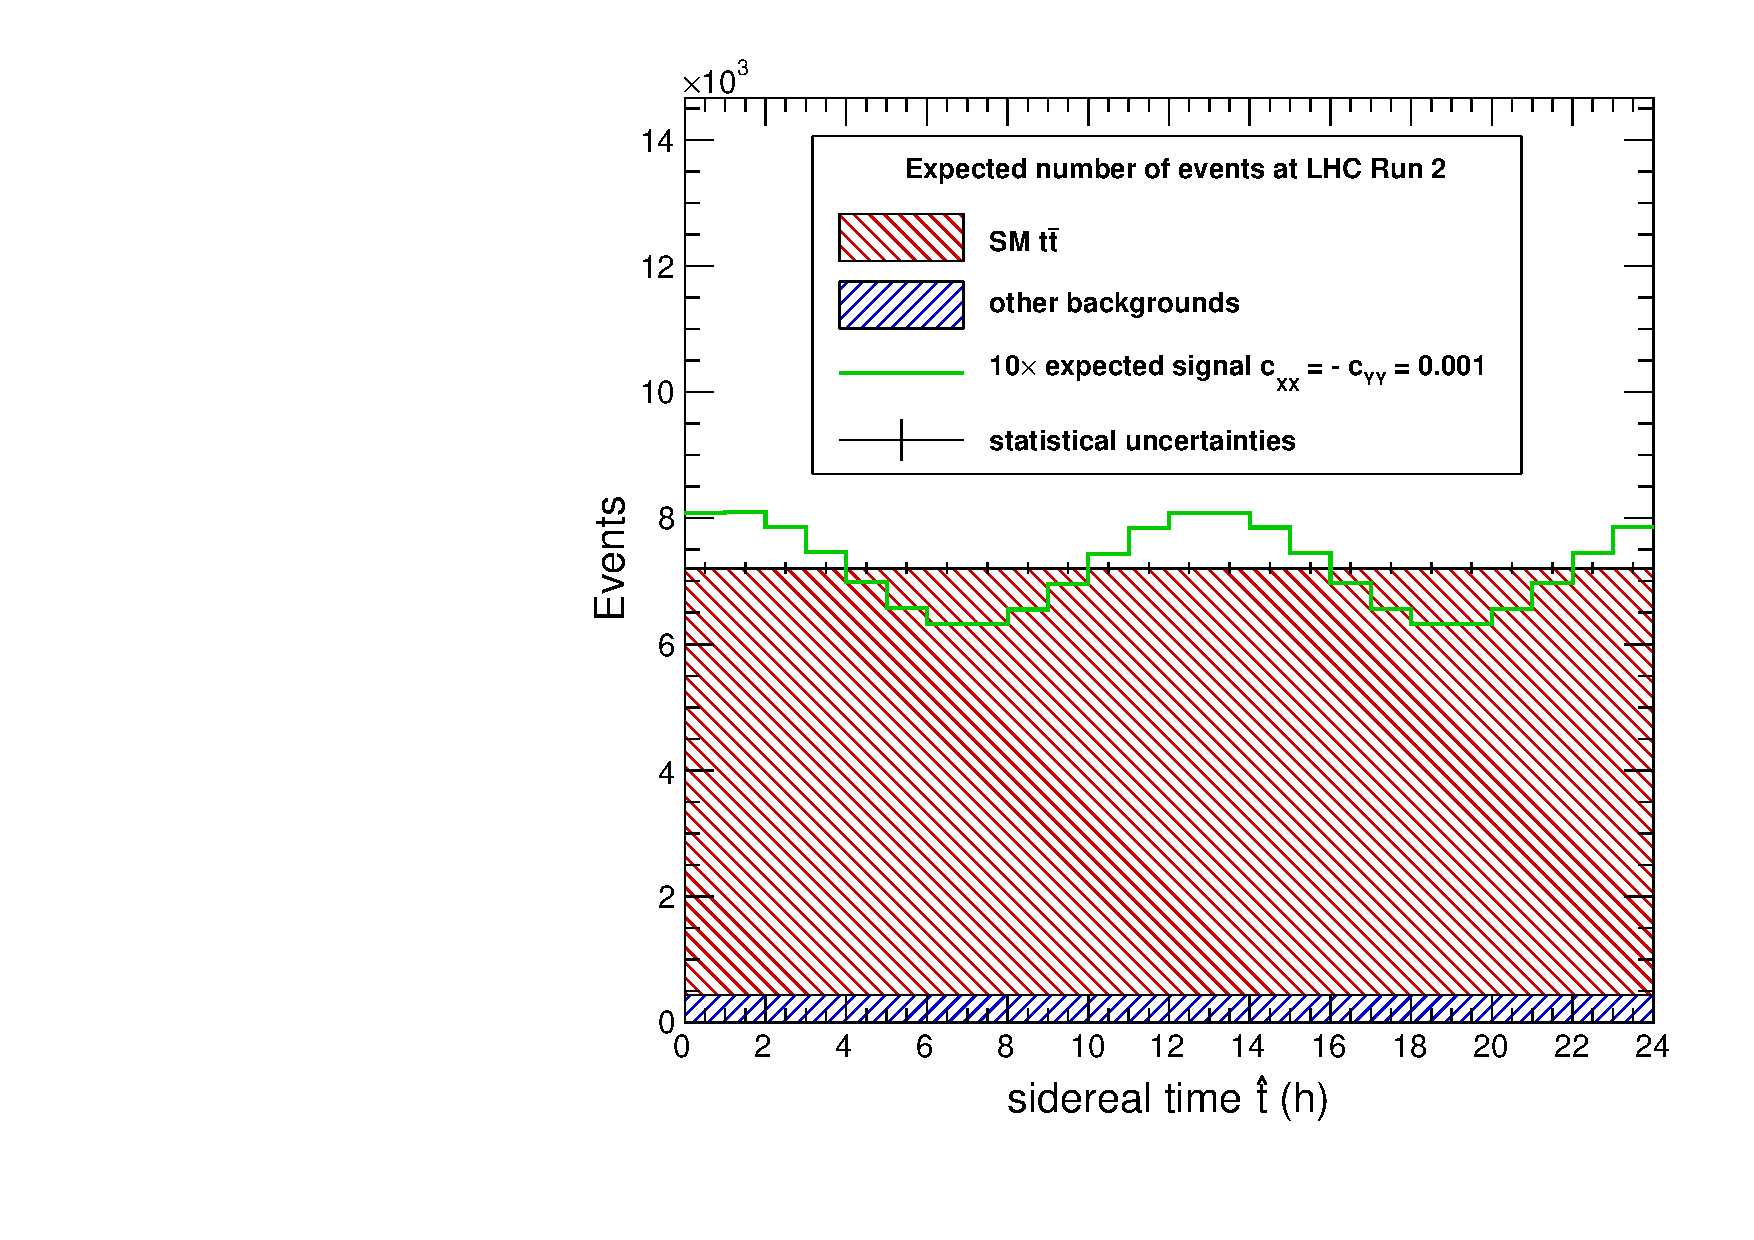
\includegraphics[scale=0.4, angle=-90]{Updated.pdf}
        \caption{Distribution du nombre d'évènements \ttbar avec 1 bin pour 1 heure sidérale \cite{Carle_2020}.}
        \label{principeanalyse}
    \end{center}
\end{figure}

\subsubsection{Le nombre d'événements attendu à CMS}

Pour évaluer le nombre d'événements de signal et de bruit de fond, nous utilisons les valeurs publiées par la collaboration CMS et présentes dans \cite{Khachatryan_2017}. Cet article présente cependant des nombres d'évènements observés pour une luminosité $\mathcal{L} = \SI{2.2}{\per\fb} $ à $\sqrt{s}= \SI{8}{TeV}$. Une projection pour atteindre la luminosité du Run II ($\mathcal{L} =\SI{150}{\per\fb} $ à $\sqrt{s}= \SI{13}{TeV}$) est nécessaire. Les valeurs après correction sont présentées dans la table \tablename{\ref{tab:cmsobserved}}.
\begin{table}
    \begin{center}
        \begin{tabular}{c|c}
            \noalign{\smallskip}\hline\noalign{\smallskip}
                    & Nombre d'événements  \\ 
             Source & \Pepm \Pmump (\SI{150}{\per\fb}) \\
            \noalign{\smallskip}
            \hline \hline
            \noalign{\smallskip}
            Bruit de fond total & \SI[parse-numbers=false]{44405 \pm 750 (stat) \pm 13322 (syst)}{}  \\
            Signal \ttbar& \SI[parse-numbers=false]{676431 \pm 955 (stat) \pm 408 (syst)}{}\\
            \noalign{\smallskip}\hline\noalign{\smallskip}
        \end{tabular}
        \caption{Nombres d'évènements $\ttbar \rightarrow \Pbottom \Pleptonplus \Pnulepton +  \APbottom \Pleptonminus \APnulepton$ observés à CMS après projection pour le Run II du LHC ($\mathcal{L} =\SI{150}{\per\fb} $).}
        \label{tab:cmsobserved}
    \end{center}
\end{table}

\subsubsection{La précision par test $\chi^2$}

Avec \SI{2}{\%}  d'incertitude attribuée à la luminosité, \SI{4}{\%} au processus Modèle Standard \ttbar et \SI{30}{\%}  au bruit de fond, le calcul de la précision est effectué par une méthode de $\chi^2$: 
    \begin{equation}\label{chi2}
        \chi^2 = \frac{1}{N_\mathrm{bin} } \sum_{i=1}^{N_\mathrm{bin}} \frac{\left(N_{i\mathrm{,tot}} -(cf(t_i) + 1)N_{i\mathrm{,signal}} - N_{i\mathrm{,background}}\right)^2}{\sigma_i^2}
    \end{equation}
    
Avec $N_\mathrm{bin}$ le nombre de bins dans l’histogramme, $N_\mathrm{i, tot}$ le nombre total d’événements au i-ième bin, $N_\mathrm{i, signal}$ le nombre d’évènements du signal, $N_\mathrm{i, background}$ le nombre d’évènements de bruits de fonds. La fonction $f(t_i)$ représente la fonction de modulation en un bin de temps donné. $c$ représente, ici, le paramètre du test $\chi^2$, également le coefficient de Wilson à tester.

De plus, le test $\chi^2$ est dit Asimov, c'est-à-dire que l'on fait l'hypothèse que les fausses données ne contiennent que le Modèle Standard et on cherche la précision sur $c_{\mu\nu}$. Avec comme exemple le couple de coefficients $c_\mathrm{LXX} = -c_\mathrm{LYY} $, l'application de \eqref{chi2} permet de conclure que $c_\mathrm{LXX} = \SI{0}{} \SI{\pm 5.98e-4}{(stat)}$, voir la figure \figurename{\ref{chi2graph}}.

\begin{figure}
    \begin{center}
        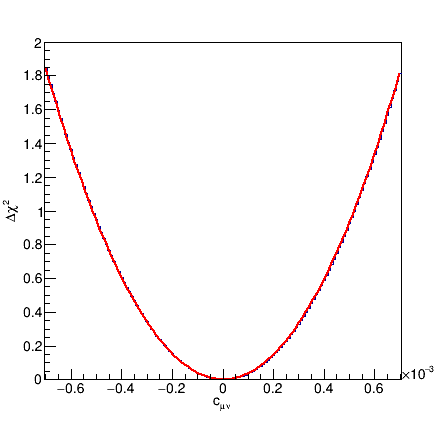
\includegraphics[scale=0.4]{X13LXX.png}
        \caption{Méthode $\chi^2$ pour l'évaluation du coefficient $c_\mathrm{LXX} = -c_\mathrm{LYY} $.}
        \label{chi2graph}
    \end{center}
\end{figure}
L’incertitude systématique est estimée avec une seconde méthode. Celle-ci consiste à directement intégrer notre incertitude systématique dans les histogrammes de signal et de bruits de fonds en faisant varier les fonds et la luminosité indépendamment. L’incertitude systématique est isolée par soustraction en quadrature \eqref{quadrature}.
\begin{equation}\label{quadrature}
    \Delta c_\mathrm{syst} = \sqrt{\left|  \Delta c^2_\mathrm{(stat+syst)} - \Delta c^2_\mathrm{(stat)}  \right| }
\end{equation}

Finalement en prenant l'incertitude systématique, on a : 
\begin{equation}
    \Delta c_\mathrm{LXX} = 0  \SI{\pm  5.98e-4}{(stat)} \SI{\pm 4.06e-4}{(syst)} < \SI{7e-4}{(stat+syst)}
\end{equation}
L'incertitude totale est prise majorée. L'ensemble des précisions attendues, dans le cadre du scenario de CMS au LHC Run II, pour les coefficient de Wilson $c_\mathrm{LXX} = -c_\mathrm{LYY} $ est résumé dans la table \tablename{\ref{limite13TeV}}.

\begin{table}
    \begin{center}
        \begin{tabular}{c|ccc}
        \hline\noalign{\smallskip}
         & Incertitudes & Incertitudes & Incertitudes  \\
         & Statistiques &  Systématiques & Totales \\
        \noalign{\smallskip}
        \hline \hline
        \noalign{\smallskip}
        $\Delta c_\mathrm{LXX} , \Delta c_\mathrm{LXY}$ & \SI{5.98e-4}{}& \SI{4.06e-4}{} & \SI{7e-4}{}\\ 
        $\Delta c_\mathrm{LXZ} , \Delta c_\mathrm{LYZ}$ & \SI{2.20e-3}{}& \SI{1.53e-3}{} &\SI{3e-3}{}\\
        \noalign{\smallskip}\hline\noalign{\smallskip}
        $\Delta c_\mathrm{RXX} , \Delta c_\mathrm{RXY}$ & \SI{2.08e-3}{} &  \SI{1.41e-3}{} & \SI{3e-3}{}\\
        $\Delta c_\mathrm{RXZ} , \Delta c_\mathrm{RYZ}$ &  \SI{7.63e-3}{} &  \SI{5.39e-3}{}& \SI{1e-2}{}\\
        \noalign{\smallskip}\hline\noalign{\smallskip}
        $\Delta c_\mathrm{XX} , \Delta c_\mathrm{XY}$& \SI{8.40e-4}{}&  \SI{5.71e-4}{} & \SI{1e-3}{}\\
        $\Delta c_\mathrm{XZ} , \Delta c_\mathrm{YZ} $&  \SI{3.09e-3}{}&  \SI{2.41e-3}{} & \SI{4e-3}{}\\
        \noalign{\smallskip}\hline\noalign{\smallskip}
        $\Delta d_\mathrm{XX} , \Delta d_\mathrm{XY}$ & \SI{4.66e-4}{}& \SI{3.12e-4}{} &\SI{6e-4}{}\\
        $\Delta d_\mathrm{XZ} , \Delta d_\mathrm{YZ}$ & \SI{1.71e-3}{}& \SI{1.21e-3}{} &\SI{2e-3}{}\\        
        \noalign{\smallskip}\hline\noalign{\smallskip}
        \end{tabular}
        \caption{Résumé de l'ensemble des incertitudes estimées pour chaque coefficient à CMS dans le scénario du Run II du LHC.}
        \label{limite13TeV}
    \end{center}
\end{table}

\subsection{Projection pour les collisionneurs futurs}

\subsubsection{L'influence de l'énergie au centre de masse}
Une première étude à mener est l'influence de $\sqrt{s}$ sur les valeurs $ \langle A_{\mu\nu} \rangle $ donc sur l'amplitude de modulation $||f(t)||$. Un nouvel ensemble de simulations \texttt{MadGraph\_aMC@NLO} \cite{Madgraph} est utilisé dont les caractéristiques sont résumées dans la table \tablename{\ref{simu}}.

\begin{table}
\begin{center}
    \begin{tabular}{c|ccc}
    \noalign{\smallskip}\hline\noalign{\smallskip}
    Scenario&Énergie au centre & Nombre & Type de  \\
    simulé&de masse & d'évènements & collisions  \\
        \noalign{\smallskip}
        \hline \hline
        \noalign{\smallskip}
    Tevatron&\SI{1.96}{\TeV}& \SI{1e6}{} &\Pproton{}-\APproton \\
    LHC RunII&\SI{13}{\TeV}& \SI{5e6}{} &\Pproton{}-\Pproton{} \\
    HL-LHC&\SI{14}{\TeV}& \SI{1e6}{} &\Pproton{}-\Pproton{} \\
    HE-LHC&\SI{27}{\TeV}& \SI{1e6}{}&\Pproton{}-\Pproton{} \\
    FCC&\SI{100}{\TeV}& \SI{1e6}{} &\Pproton{}-\Pproton{} \\
    \noalign{\smallskip}\hline\noalign{\smallskip}
    \end{tabular}
    \caption{Caractéristiques des simulations  $\ttbar \rightarrow \Pbottom \Pleptonplus \Pnulepton +  \APbottom \Pleptonminus \APnulepton$ avec \texttt{MadGraph5}}
    \label{simu}
\end{center}
\end{table}

Le résultat montre une évolution de l'amplitude de modulation avec l'énergie au centre-de-masse. Cette évolution est visible sur la figure \figurename{\ref{fig:amplitudeenergy}}.

\begin{figure}
    \begin{center}
        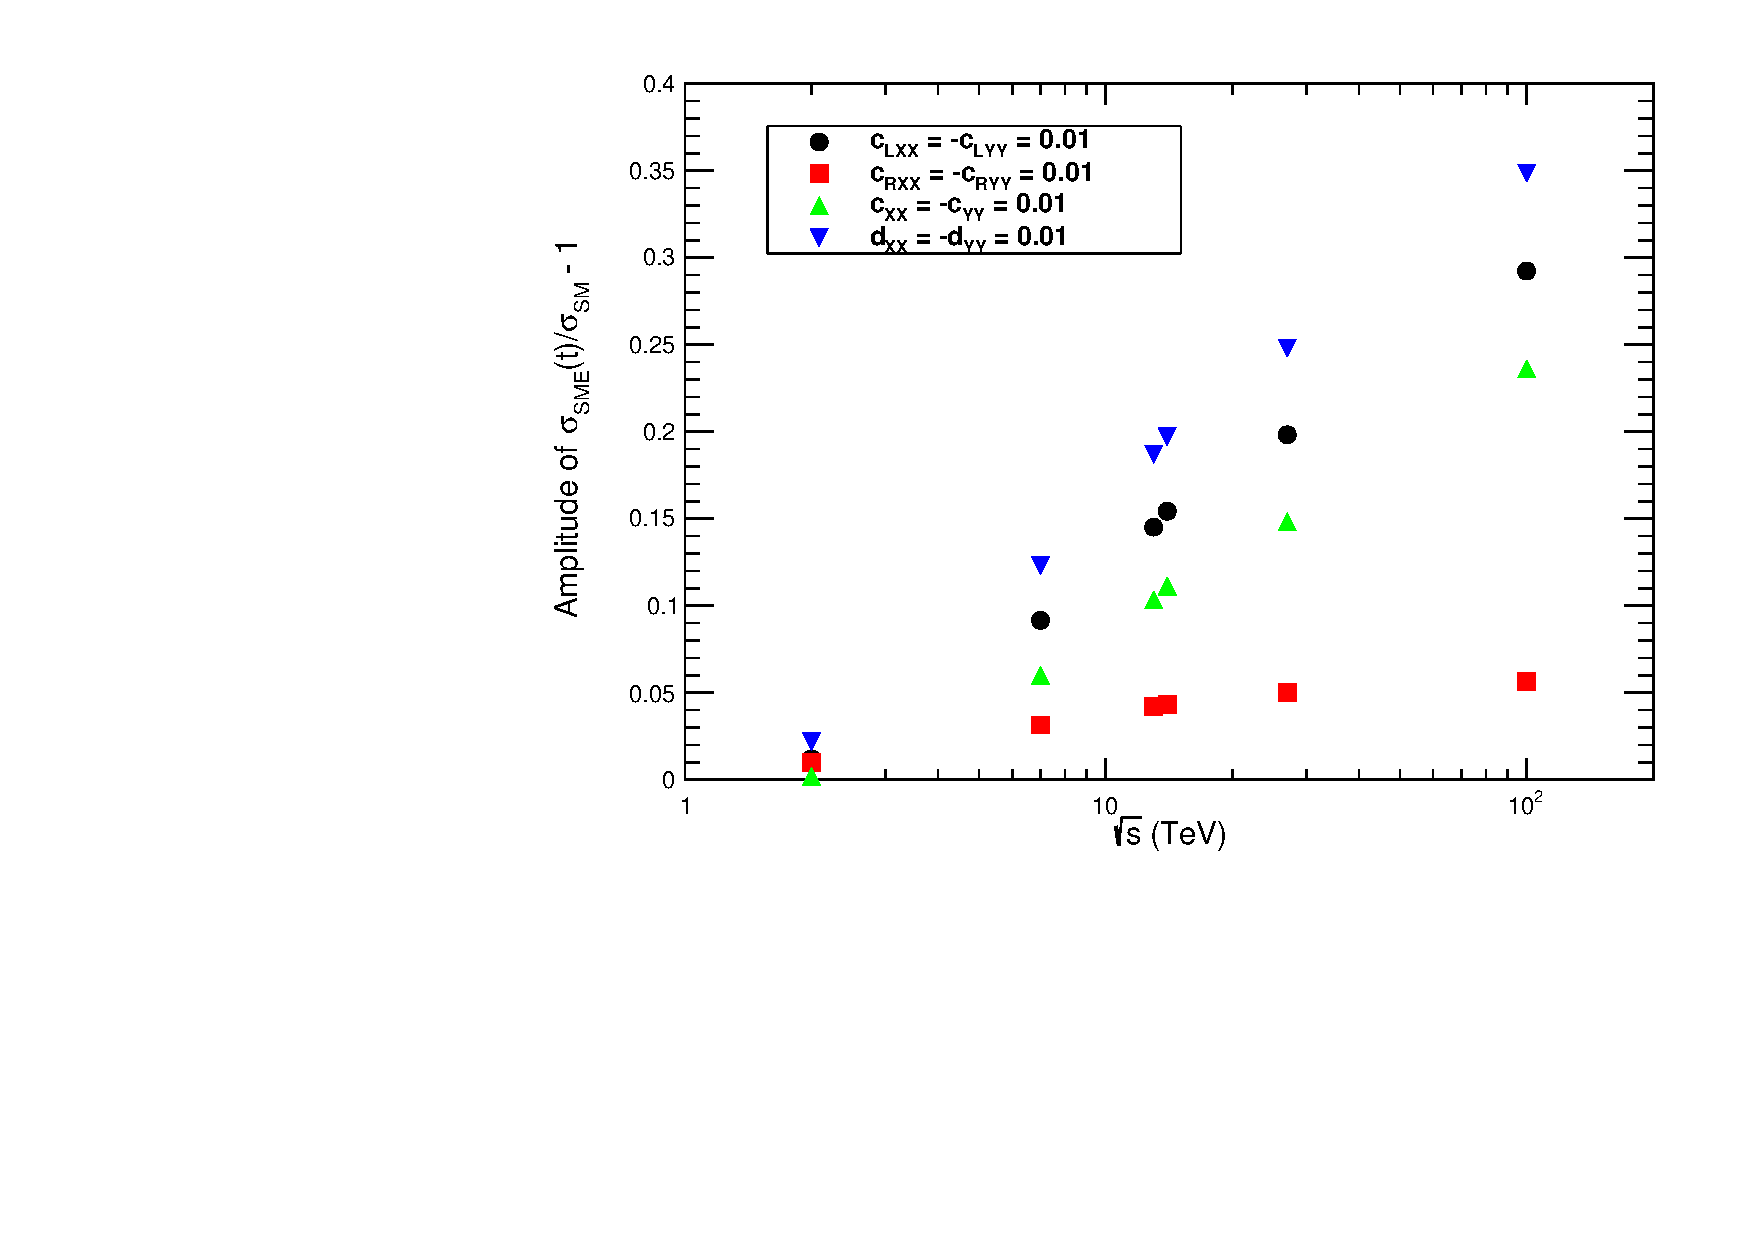
\includegraphics[width=0.6\textwidth, angle=-90]{energy.pdf}
        \caption{Amplitude de $f(t)$ pour le Tevatron, LHC, HL-LHC, HE-LHC et FCC, pour $c_\mathrm{XX}= −c_\mathrm{YY} = 0.01 $ \cite{Carle_2020}.}
        \label{fig:amplitudeenergy}
    \end{center}
\end{figure}

Cette fonction de $\sqrt{s}$ montre une forme en racine carrée. Une telle tendance n'étant pas explicitement présente dans les équations des éléments de matrice du SME, une étude plus approfondie a été entreprise. 
En effet, en reprenant les équations complètes des éléments de matrice présentes dans \cite{KosteleckyPheno}, on peut voir une tendance parabolique de ces quantités en fonction de l'énergie au centre-de-masse. Avec une nouvelle génération de simulation avec les  caractéristiques de la table \tablename{\ref{simu}} mais avec l'absence de PDF, nous avons pu découvrir une tendance parabolique comme présentée dans la figure \figurename{\ref{parabole}}. 
Ainsi, nous avons conclu que c'est l'effet des PDF qui donne à l'évolution de l'amplitude d'oscillation en fonction de $\sqrt{s}$ cette tendance en racine carrée.


\begin{figure}
    \begin{center}
        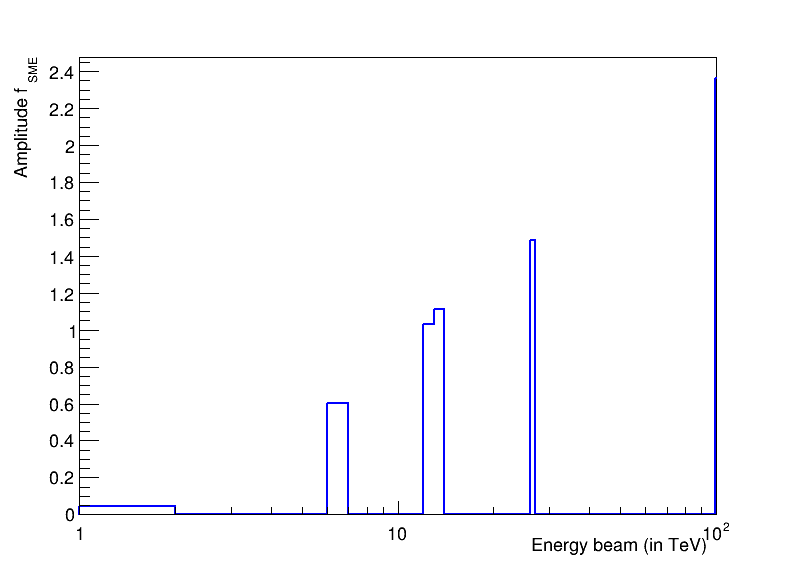
\includegraphics[scale=0.4]{CArticle.png}
        \caption{Amplitude de $f(t)$ pour le Tevatron, LHC, HL-LHC, HE-LHC et FCC, pour $c_\mathrm{LXX}= −c_\mathrm{LYY} = 0.01 $, pour des évènements générés sans PDF.}
        \label{parabole}
    \end{center}
\end{figure}

\subsubsection{L'influence de l'orientation du détecteur}

Un paramètre intéressant dans la valeur de l'amplitude de modulation est l'orientation du détecteur. En effet, en reprenant les variables de latitude $\lambda$ et d'azimut $\theta$, nous pouvons observer des zones de différences d'amplitude. 
Pour établir l'équation du maximum d'amplitude fonction de $\lambda$ et $\theta$, on doit commencer par trouver le temps d'amplitude maximale $t_\mathrm{max}$ puis le réintroduire dans la fonction $f$. Une démonstration approfondie se trouve en appendice \ref{B:max}.
\begin{equation}
    f'(t_\mathrm{max}) = 0
\end{equation}
Pour le cas $c_\mathrm{XX}= −c_\mathrm{YY}$ : 
\begin{equation}
    t_\mathrm{max} = \frac{1}{2\Omega} \cot^{-1} \left(\frac{a_1 - a_2}{2a_3}\right)
\end{equation}
On obtient ainsi : 
\begin{equation}\label{f2D}
    f(\lambda, \theta) = 2 c_\mathrm{XX} \left( \left(\frac{a_1 - a_2}{2}\right) \cos\left( \cot^{-1} \left(\frac{a_1 - a_2}{2a_3}\right)\right)  + a_3 \sin\left( \cot^{-1} \left(\frac{a_1 - a_2}{2a_3} \right) \right)  \right) 
\end{equation}\
En faisant un tracé 2D de la fonction \eqref{f2D}, on obtient la figure \figurename{\ref{orientation}}.

\begin{figure}
    \begin{center}
        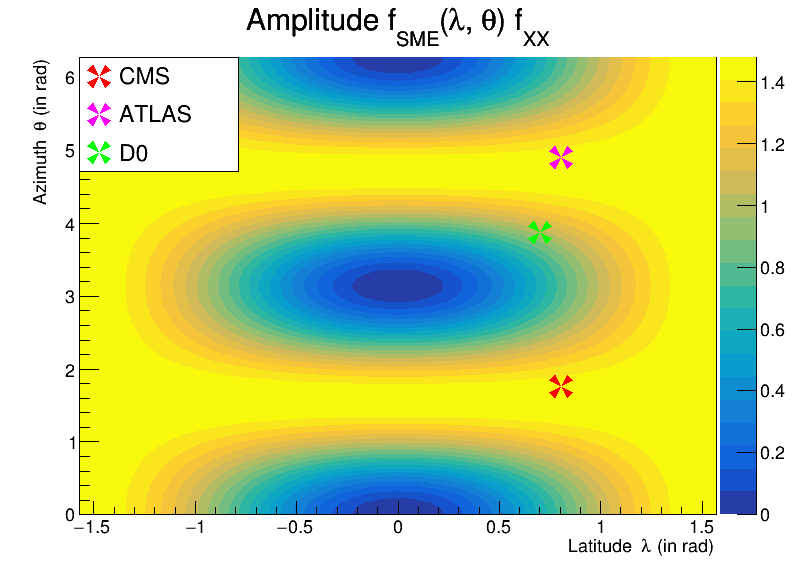
\includegraphics[scale=0.4]{XX.png}
        \caption{Amplitude de $f(\lambda, \theta)$ en fonction de la latitude et de l'azimut pour $c_\mathrm{XX}= −c_\mathrm{YY}$ dans un scénario à \SI{13}{\TeV} avec les orientations de détecteurs CMS, ATLAS et D$\emptyset$ \cite{Carle_CPT19}.}
        \label{orientation}
    \end{center}
\end{figure}

Ce résultat montre la dépendance de l'orientation du détecteur de l'amplitude d'oscillation. Dans la figure \figurename{\ref{orientation}} on observe que l'orientation du détecteur CMS, comme celle d'ATLAS offre un plus grand maximum d'oscillation que D$\emptyset$. De plus on remarque que CMS et ATLAS ont tout deux la même amplitude, ceci s'explique du fait que les deux détecteurs ont une position opposée sur l'anneau du LHC. Cette tendance est dépendante de la fonction de modulation étudiée (voir l'annexe \ref{B:orientation}).

\subsubsection{L'influence de la luminosité}

Finalement la dernière influence majeure pour l'estimation des limites sera la luminosité, autrement dit le nombre d'évènements mesurés. Elle augmentera la précision d'un facteur \sfrac{1}{$\sqrt{N}$}.

La dernière étape consiste à extrapoler linéairement les valeurs du nombre d'événements pour les futurs collisionneurs. 
En utilisant la même méthode de $\chi^2$ présentée en \eqref{chi2}, une table des précisions attendues sur les coefficients de Wilson de la partie cinétique du SME dans le secteur du quark top a été dressée dans le tableau \tablename{\ref{CarleResults}}.

\begin{table}[H]
    \begin{center}
    \begin{tabular}{c|ccccc}
        \hline\noalign{\smallskip}
         &  D$\emptyset$  & LHC (Run II)  & HL-LHC  & HE-LHC & FCC\\
        \noalign{\smallskip}
        \hline \hline
        \noalign{\smallskip}
        $\Delta c_\mathrm{LXX} , \Delta c_\mathrm{LXY}$ & \SI{1e-1}{}  & \SI{7e-4}{} & \SI{2e-4}{} & \SI{2e-5}{} & \SI{5e-6}{} \\
        $\Delta c_\mathrm{LXZ} , \Delta c_\mathrm{LYZ}$ & \SI{8e-2}{} & \SI{3e-3}{} & \SI{5e-4}{} & \SI{8e-5}{} & \SI{2e-5}{} \\
        \noalign{\smallskip}\hline\noalign{\smallskip}
        $\Delta c_\mathrm{RXX} , \Delta c_\mathrm{RXY}$ & \SI{9e-2}{}  & \SI{3e-3}{} & \SI{5e-4}{} & \SI{8e-5}{} & \SI{5e-5}{} \\
        $\Delta c_\mathrm{RXZ} , \Delta c_\mathrm{RYZ}$ & \SI{7e-2}{} & \SI{1e-2}{} & \SI{2e-3}{} & \SI{4e-4}{} & \SI{8e-5}{} \\
        \noalign{\smallskip}\hline\noalign{\smallskip}
        $\Delta c_\mathrm{XX} , \Delta c_\mathrm{XY}$ & \SI{7e-1}{}  & \SI{1e-3}{} & \SI{2e-4}{} & \SI{3e-5}{} & \SI{9e-6}{} \\
        $\Delta c_\mathrm{XZ} , \Delta c_\mathrm{YZ}$ & \SI{6e-1}{} & \SI{4e-3}{} & \SI{7e-4}{} & \SI{1e-4}{} & \SI{3e-5}{} \\
        \noalign{\smallskip}\hline\noalign{\smallskip}
        $\Delta d_\mathrm{XX} , \Delta d_\mathrm{XY}$ & \SI{1e-1}{}  & \SI{6e-4}{} & \SI{1e-4}{} & \SI{2e-5}{} & \SI{8e-6}{} \\
        $\Delta d_\mathrm{XZ} , \Delta d_\mathrm{YZ}$ & \SI{7e-2}{} & \SI{2e-3}{} & \SI{4e-4}{} & \SI{8e-5}{} & \SI{2e-5}{} \\
        \noalign{\smallskip}\hline\noalign{\smallskip}
    \end{tabular}
    \caption{Précisions attendues sur les coefficients de Wilson de la partie cinétique du SME dans le secteur du quark top pour différents scenarii de collisionneurs.}
    \label{CarleResults}
    \end{center}
\end{table}

Il est à noter que par rapport à l'expérience D$\emptyset$ du Tevatron une augmentation majeure de la précision est attendue, de l'ordre de $\num{e2}$ à $\num{e3}$ pour le RunII du LHC. Un gain de précision de l'ordre de  $\num{e5}$ à $\num{e6}$ pour le scénario du FCC-hh est également prévu. Cette étude de faisabilité nous encourage à procéder à cette analyse dans les données de CMS au Run II.

Un résumé de ces résultats est disponible dans la publication de "The European Physical Journal C" : \textbf{Prospects for Lorentz invariance violation searches with top pair production at the LHC and future hadron colliders.}\cite{Carle_2020}

\section{Conclusion}

Finalement, nous avons vu que le secteur du quark top possède dans le cadre du SME des propriétés qui rendent riches les exploitations phénoménologiques. Du fait de l'utilisation du SCF comme référentiel privilégié, une étude sur le changement de référentiel a été nécessaire. Premièrement une compréhension des différentes définitions de temps a d\^u être clarifiée. Deuxièmement la rotation qui nous sert de matrice de passage entre le SCF et CMS a due être construite. Grâce à la rotation de la Terre par rapport au SCF, on a pu dégager un signal caractéristique d'une modulation au cours du temps.
Nous avons, ensuite, pu montrer que la modulation voyait son amplitude dépendre de l'énergie au centre-de-masse de la collision et de l'orientation du détecteur. Ainsi, nous avons pu faire une estimation des précisions attendues pour l'observation de la section efficace dans divers scenarii de collisionneurs. Cette précision toujours croissante avec les nouvelles générations de collisionneur est allée jusqu'à améliorer d'un facteur $\num{e5}$ à $\num{e6}$ la mesure expérimentale de l'expérience D$\emptyset$ au Tevatron.


\end{fmffile}
